\documentclass[10pt,a4paper]{article}

\usepackage{amsmath}
\usepackage{amsthm}
\usepackage{amsfonts} % unneccesary if amssymb loaded
\usepackage{amssymb} % unneccesary if amsfonts loaded

\usepackage[textwidth=14cm,
textheight=22cm,
centering]{geometry}

%% The consecutive references should be cited as ex. [4-9]:
\usepackage[noadjust]{cite}

\usepackage{tikz}

%\usepackage{url}
\usepackage{hyperref}

%--- ONLY FOR DRAFTS  (or to mark changes)
%\usepackage{color}
%\newcommand{\rojo}[1]{\textcolor{red}{#1}}
%\newcommand{\azul}[1]{\textcolor{blue}{#1}}

%--- ONLY FOR DRAFTS (put it after hyperref)
%\usepackage{backref}
%\usepackage{refcheck}
%\usepackage[notcite,notref]{showkeys}

\usepackage{graphicx}

%\usepackage{tikz}

%--- \allowdisplaybreaks es una orden de amsmath que permite cortes de
%--- p\'agina dentro de una f\'ormula de varias l\'ineas (align, multline, gather,...)
\allowdisplaybreaks[3]
%--- Escala de 1 (permite algo) a 4 (ninguna traba para cortar).
%--- Si en alg\'un sitio queremos impedir un posible corte, basta usar \\* en vez de \\

\numberwithin{equation}{section}

\theoremstyle{plain}
\newtheorem{Theo}{Theorem}[section]
\newtheorem{Cor}[Theo]{Corollary}
\newtheorem{Lem}[Theo]{Lemma}

\theoremstyle{definition}
\newtheorem{Conjecture}{Conjecture}[section]

%\theoremstyle{definition}
%\newtheorem*{Def}{Definition}

%\theoremstyle{remark}
%\newtheorem{Rem}{Remark}
%\newtheorem{Claim}{Claim}

\newcommand{\I}{\mathcal{I}}
\newcommand{\aA}{\mathfrak{a}}
\newcommand{\dd}{\mathfrak{d}}
\newcommand{\cc}{\gamma}
%\newcommand{\K}{\mathcal{K}}

\newcommand{\RR}{\mathbb{R}}
%\newcommand{\ZZ}{\mathbb{Z}}
\newcommand{\NN}{\mathbb{N}}
\newcommand{\CC}{\mathbb{C}}
\newcommand{\ZZO}{\mathbb{Z} \setminus \{0\}}

\renewcommand{\Im}{\operatorname{Im}}
\renewcommand{\Re}{\operatorname{Re}}
\newcommand{\sign}{\operatorname{sign}}

%------
%--- Definitions for the functions pFq.
%--- In this way is only for 2F1
%--- (for general pFq it is enough to use to extra parameters).
%--- Version for displaymath:
\newcommand{\FF}[3]{{}_{2}F_{1}\bigg(\genfrac{}{}{0pt}{}{#1}{#2};#3\bigg)}
% Version for text:
\newcommand{\tFF}[3]{{}_{2}F_{1}\Big(\genfrac{}{}{0pt}{}{#1}{#2};#3\Big)}
%------

%----------
\title{On the properties of zeros of Bessel series in the real line}
%----------

%----------
\author{Antonio J. Dur\'an\textsuperscript{1},
Mario P\'erez\textsuperscript{2}
and Juan L. Varona\textsuperscript{3}\\[6pt]
\small\textsuperscript{1}Departamento de An\'alisis Matem\'atico and IMUS,
Universidad de Sevilla,\\[-2pt]
\small 41080 Sevilla, Spain. Email: {duran@us.es}\\[6pt]
\small\textsuperscript{2}Departamento de Matem\'aticas and IUMA,
Universidad de Zaragoza,\\[-2pt]
\small 50009 Zaragoza, Spain. Email: {mperez@unizar.es}\\[6pt]
\small\textsuperscript{3}Departamento de Matem\'aticas y
Computaci\'on, Universidad de La Rioja,\\[-2pt]
\small 26006 Logro\~no, Spain. Email: {jvarona@unirioja.es}}
%----------

%%----------
%\author{
%\name{Antonio J. Dur\'an\textsuperscript{a},
%Mario P\'erez\textsuperscript{b}
%and Juan L. Varona\textsuperscript{c}}
%\affil{\textsuperscript{a}Departamento de An\'alisis Matem\'atico and IMUS,
%Universidad de Sevilla, Sevilla, Spain, {duran@us.es};\\
%\textsuperscript{b}Departamento de Matem\'aticas and IUMA,
%Universidad de Zaragoza, Zaragoza, Spain, {mperez@unizar.es};\\
%\textsuperscript{c}Departamento de Matem\'aticas y Computaci\'on,
%Universidad de La Rioja, Logro\~no, Spain, {jvarona@unirioja.es}}
%}
%%----------

\date{}

%----------
\begin{document}
%----------

\makeatletter
\def\blfootnote{\gdef\@thefnmark{}\@footnotetext}
\makeatother
\blfootnote{\textbf{This paper has been published as:}
Antonio J. Dur\'an, Mario P\'erez and Juan L.~Varona, 
On the properties of zeros of Bessel series in the real line,
\textit{Integral Transforms Spec.\ Funct.}\ \textbf{32} (2021), no.~11, 912--931, 
\url{https://doi.org/10.1080/10652469.2020.1867129}}

%\articletype{Research Article}% Specify the article type or omit as appropriate
%\articletype{Integral Transforms Spec. Funct.
%\textbf{32} (2021), no.~11, 912--931\\
%doi: 10.1080/10652469.2020.1867129}

%----------
\maketitle
%----------

%----------
\begin{abstract}
For a given sequence of real numbers $\mathfrak{a} = (a_m)_{m\ge 1}$, we define the function
\[
   U_{\mu,\nu}^{\mathfrak{a}}(x) = \frac{2^\mu\Gamma(\mu+1)}{x^\mu}
   \sum_{m\ge 1} \frac{a_m}{j_{m,\nu}^\mu}J_\mu (j_{m,\nu} x),
   \quad x\in (0,+\infty),
\]
where $\mu,\nu>-1$, $J_\mu$ denotes the Bessel function of order~$\mu$, and $(j_{m,\nu})_{m\geq 1}$ are the positive zeros of~$J_\nu$.
In this paper, we study the function $U_{\mu,\nu}^{\mathfrak{a}}$ and some outstanding instances of it on the whole real line and propose a number of conjectures about its positive zeros.

\medskip
\noindent 
\textbf{Keywords:} Bessel functions, zeros, Bessel series.

\medskip
\noindent 
\textbf{2010 Mathematics Subject Classification:} Primary 33C10; Secondary 42C10, 34C10.
\end{abstract}

%\begin{keywords}
%Keywords: Bessel functions, zeros, Bessel series.
%\end{keywords}

%% 2010 Mathematics Subject Classification: Primary 33C10; Secondary 42C10, 34C10.
%\begin{amscode}
%Primary 33C10; Secondary 42C10, 34C10.
%\end{amscode}
%----------

%----------
\section{Introduction}
%----------

For $\nu>-1$, consider the Bessel function $J_\nu$ of order~$\nu$. The zeros $j_{m,\nu}$ ($m=1,2,\dots$) of the Bessel function $J_{\nu}$ are positive and can be ordered so that $0<j_{m,\nu}< j_{m+1,\nu}$, $m\ge 1$ (\cite[\S\,15.27, p.~483]{Wat}).

Let $\aA=(a_m)_{m\ge 1}$ be a sequence of real numbers satisfying
\begin{equation}
\label{eq:pcs}
   \sum _{m=1}^\infty \frac{|a_m|}{j_{m,\nu}^{\mu+1/2}} < +\infty,
   \quad
   \sum _{m=1}^\infty |a_m| < +\infty,
\end{equation}
where $\mu,\nu>-1$. We then define the function
\begin{equation}
\label{eq:gfs}
   U_{\mu,\nu}^{\aA}(x) = \frac{2^\mu\Gamma(\mu+1)}{x^\mu}
   \sum_{m\ge 1} \frac{a_m}{j_{m,\nu}^\mu}J_\mu (j_{m,\nu} x),
   \quad x\in (0,+\infty).
\end{equation}
Using well-known bounds for the Bessel functions (see Section~\ref{sec:Sonine} below), it is easy to show that the Bessel series \eqref{eq:gfs} defines a continuous function $U_{\mu,\nu}^\aA$ on $[0,+\infty)$. Since $J_\mu(x)/x^\mu$ is an even function, we can
extend the function $U_{\mu,\nu}^\aA$ to $(-\infty,0)$ just by setting $U_{\mu,\nu}^\aA(x)=U_{\mu,\nu}^\aA(-x)$.

For particular values of the parameters $\mu$ and $\nu$, and except for the factor $1/x^\mu$, the series \eqref{eq:gfs} are examples of Fourier series in $[0,1]$:
\begin{enumerate}
\item Sine or cosine orthogonal series for $\nu=\pm 1/2$, $\mu=\pm 1/2$ (for these values, $j_{m,1/2}=m\pi$ and $j_{m,-1/2} = (2m-1)\pi/2$).
\item Fourier-Bessel series for $\mu=\nu$.
\item Dini series for $\mu=\nu+1$.
\item Schl\"{o}milch series for $\nu=1/2$. They are not properly Fourier series but have enough similarities with them so as to be considered Fourier type series.
\end{enumerate}
All these Fourier series have been studied in the bounded interval $[0,1]$ where the orthogonality occurs.

For the particular values of $\mu=\nu=1/2$ the function
\begin{equation}
\label{eq:funu}
   xU_{1/2,1/2}^\aA(x) = \sum_{m\ge 1} \frac{a_m}{m\pi}\sin(m\pi x)
\end{equation}
is odd and periodic, with period $2$. As a consequence, since $xU_{1/2,1/2}^\aA(x)$ vanishes at $x=0,1$, the function $U_{1/2,1/2}^\aA(x)$ vanishes at each interval $[k,k+1)$, $k\ge 1$ (to be precise, it vanishes at $k$). As the main result in this paper, we prove that this fact is essentially true when
the periodicity disappears.
We stress that we are interested in the zeros of $U_{\mu,\nu}^\aA$ on the whole real line, and hence our results are rather different to the aim of the theorem of P\'olya-Szeg\H{o} on trigonometric polynomials \cite[Th.~6.4, p.~134]{Sz} or similar results.

The content of this paper is as follows.
In Section~\ref{sec:kernel}, we study the case $\nu=1/2$ (when $j_{m,\nu}=m\pi$). We then write the function $U_{\mu,1/2}^{\aA}$, $\mu>1/2$, as an integral transform of the periodic function $vU_{1/2,1/2}^\aA(v)$, $v\in[0,1]$, with respect to a suitable kernel $K_\mu:[0,\infty)\times [0,1]\to \RR$ (see~\eqref{def:kerpar} and~\eqref{def:kerimpar} below):
\[
   U_{\mu,1/2}^{\aA}(x)
   = \frac{4\Gamma(\mu+1)}{\sqrt{\pi} \, \Gamma(\mu-1/2)x^{2\mu}}
   \int_0^1 v U^\aA_{1/2,1/2}(v) K_\mu(x,v)\,dv.
\]
It turns out that for $\mu > 1/2$ and $x=k\in \NN$ big enough (depending on $\mu$) the kernel $K_{\mu}(k,v)$ has a constant sign in $[0,1]$ which oscillates with $k$. This allows us to prove the following theorem:

%---
\begin{Theo}
\label{theo:U1/2}
Assume that the function $vU_{1/2,1/2}^{\aA}(v)$ defined in \eqref{eq:funu}
has constant sign for $v\in (0,1)$. Then, for each $\mu > 1/2$ there exists some integer $k_{\mu}$ (which does not depend on the sequence~$\aA$) such that the function $U_{\mu,1/2}^{\aA}$ defined in \eqref{eq:gfs} has at least one zero in each interval $[k,k+1)$, for $k\in \NN$, $k\ge k_{\mu}$. In particular, for $1/2 < \mu \le 5/2$, we can take $k_{\mu}= 1$.
\end{Theo}

We guess that Theorem~\ref{theo:U1/2} is also true for $\mu>-1$ without any additional assumption. This question and other related ones will be considered in Section~\ref{sec:zerosU}, where we propose a number of conjectures about the positive zeros of $U_{\mu,\nu}^{\aA}$. For instance, the quantification of the number of zeros of the function $U_{\mu,1/2}^{\aA}$ on an interval $[k,k+1)$ is a difficult challenge which seems to depend not on how many changes of sign $vU_{1/2,1/2}^{\aA}(v)$ has on $(0,1)$ but on its shape. Surprisingly, however, there are several properties of the zeros of $U_{\mu,1/2}^{\aA}$ which seem to be more regular when $\mu$ is big enough.

%---
\begin{Conjecture}
\label{conj:onezero}
There exists some $\mu_0>-1$ satisfying that for any $\mu\ge \mu_0$ there exists some nonnegative integer $k_\mu$ (depending only on $\mu$) such that if $vU_{1/2,1/2}^{\aA}(v)$ has constant sign in $(0,1)$, then:
\begin{enumerate}
\item The function $U_{\mu,1/2}^{\aA}$ has exactly one simple zero in each interval $[k,k+1)$, for $k\ge k_\mu$.
\item The zeros of $U_{\mu,1/2}^{\aA}$ separate the zeros of $U_{\mu+1,1/2}^\aA$ in $[k_\mu ,+\infty)$.
\item If $\mu_0\le\nu\le \mu$ then the $m$-th zero of $U_{\nu,1/2}^{\aA}$ in $[k_\mu,+\infty)$ is an increasing function of $\nu$.
\end{enumerate}
\end{Conjecture}

Our computational evidences show that $\mu_0$ could be a relatively small number: $\mu_0=12$ seems to be enough.

In Section~\ref{sec:funV}, we introduce the functions $V_{\mu,\nu}^b$ as
\begin{equation}
\label{eq:gfs1}
   V_{\mu,\nu }^{b}(x) = \frac{2^{\mu-\nu}\Gamma(\mu+1)}{\Gamma(\nu+1)x^\mu}
   \sum_{m\ge 1} \frac{J_\mu (j_{m,\nu} x)}{j_{m,\nu}^{b+\mu-\nu} J_{\nu+1}(j_{m,\nu})},
\end{equation}
where $b>\max\{\nu-\mu+1,\nu+3/2\}$. They are particular cases of the functions $U_{\mu,\nu}^\aA$ for
\[
   a_m = \frac{2^{-\nu}}{j_{m,\nu}^{b-\nu} \Gamma(\nu+1)J_{\nu+1}(j_{m,\nu})}.
\]
We study the functions $V_{\mu,\nu}^b$ when $b$ is an odd integer. It has been known for a long time that $V_{\mu,\mu}^{1}(x)$ is constant on the interval $[0,1]$, see \cite[18.12(1), p.~581]{Wat}. Using residues as the main tool, we will prove that actually each function $V_{\mu,\nu}^{2n+1}$, $n=0,1,2,\dots$, is a polynomial of degree $2n$ on the interval $[0,1]$, and provide a recurrence relation to compute explicitly this sequence of polynomials. Using the Sonine formula for Bessel functions, we also find an explicit expression for $V_{\mu,1/2}^{2n+1}(x)$, $n=0,1,2,\dots$, outside $[0,1]$ in terms of a hypergeometric function. We prove that the function $V_{1/2,1/2}^{2n+1}$ satisfies the hypothesis of Theorem~\ref{theo:U1/2}; hence, $V_{\mu,1/2}^{2n+1}$ has at least one zero on each interval $[k,k+1)$ for $k$ big enough (depending only on $\mu$; for $1/2 < \mu \le 5/2$ this function actually has at least one zero on each interval $[k,k+1)$ for $k\ge 1$).

The zeros of special functions are an integral part of the approximation theory and some other related areas such as numerical integration (\cite{Temme-NIST}), or orthogonal and hypergeometric polynomials (\cite[Ch.~VI]{Sz}, \cite{DJM, MR, Cer, JWZ, DPVW, DMu} and references therein). As pointed out above, our functions $U_{\mu,\nu}^{\aA}$ are closely related to some outstanding orthogonal systems on the interval $[0,1]$, but we are interested in the zeros of these functions outside this interval, where, as we have shown, some remarkable regularities seem to appear.
We emphasize something that will be apparent to any reader of this paper:
the full picture of these regularities is still far from being complete. This
paper is a first attempt to pose some new questions about zeros of special functions
and rise a number of conjectures (for which we have extensive computational evidence) which show the richness of the situation at hand.

%----------
\section{A Sonine formula for the functions $U_{\mu,\nu}^\aA$}
\label{sec:Sonine}
%----------

For each $\mu > -1$, there exists some constant $C_{\mu} > 0$ such that
\begin{equation}
\label{eq:cotaJa}
   | J_{\mu}(x) | \leq
   \begin{cases}
   C_{\mu} |x|^{\mu}, &\mbox{if } \quad |x| \leq 1,
   \\
   C_{\mu} |x|^{-1/2}, &\mbox{if } \quad |x| \geq 1
   \end{cases}
\end{equation}
(see~\cite[3.1(8), p.~40]{Wat} and~\cite[7.21(1), p.~199]{Wat}, or~\cite[formulas 10.7.3 and 10.7.8]{OlMa-NIST}). Since $j_m \sim m$ as $m \to \infty$ (see~\cite[\S\,15.53, p.~506]{Wat}), the series in \eqref{eq:gfs} converges uniformly on every compact set in $[0,+\infty)$ under the condition \eqref{eq:pcs}, so that $U_{\mu,\nu}^\aA(x)$ is well defined and continuous on $[0,+\infty)$.

The object of this section is to prove the formula
\begin{equation}
\label{eq:sonin-U}
   U_{\mu,\nu}^\aA(x) = 2(\mu-\eta)\binom{\mu}{\eta}
   \int_0^1 U_{\eta,\nu}^\aA(xs) s^{2\eta+1} (1-s^2)^{\mu-\eta-1} \, ds,
\end{equation}
for $\mu > \eta > -1$ and $\nu > -1$, provided that
\begin{equation}
\label{eq:pcs-eta}
   \sum_{m\geq 1} \frac{|a_m|}{j_{m,\nu}^{\eta + 1/2}} < +\infty,
   \qquad
   \sum _{m=1}^\infty |a_m| < +\infty
\end{equation}
(which is the condition required to define $U_{\eta,\nu}^\aA$ and implies \eqref{eq:pcs}).
This formula is an analogue of Sonine's formula
\begin{equation}
\label{eq:sonin}
   J_{\mu+\nu+1}(z) = \frac{z^{\nu+1}}{2^\nu \Gamma(\nu+1)}
   \int_0^1 J_\mu(zs) s^{\mu+1} (1-s^2)^\nu \, ds,
\end{equation}
valid for $\mu, \nu \in \CC$, $\Re \mu > -1$, $\Re \nu > -1$ (\cite[12.11(1), p.~373]{Wat}, after a change of variable $s = \sin \theta$).

Given $x > 0$, the definition \eqref{eq:gfs} gives
\begin{multline*}
   2(\mu-\eta)\binom{\mu}{\eta}
   \int_0^1 U_{\eta,\nu}^\aA(xs) s^{2\eta+1} (1-s^2)^{\mu-\eta-1} \, ds
   \\
   = \frac{2^{\nu+1}\Gamma(\mu+1)}{\Gamma(\mu-\eta)}
   \int_0^1
   \frac{1}{(xs)^\eta} \sum_{m\geq 1} \frac{a_m}{j_{m,\nu}^\eta} J_\eta(j_{m,\nu} xs)
   s^{2\eta+1} (1-s^2)^{\mu-\eta-1} \, ds.
\end{multline*}
Commuting the series and the integral, which will be justified next, and using Sonine's identity \eqref{eq:sonin} with $\eta$ instead of $\mu$, $\mu - \eta - 1$ instead of $\nu$, and $j_{m,\nu} x$ instead of $z$ easily proves \eqref{eq:sonin-U}, under the conditions $\mu > \eta > -1$ and $\nu > -1$.

Now, commuting the series and the integral is justified if
\[
   \sum_{m\geq 1} \frac{|a_m|}{j_{m,\nu}^\eta}
   \int_0^1 \frac{1}{(xs)^\eta}
   |J_\eta(j_{m,\nu} xs)|
   s^{2\eta+1} (1-s^2)^{\mu-\eta-1} \, ds
   < +\infty.
\]
The bounds \eqref{eq:cotaJa} give
\begin{multline*}
   \sum_{m\geq 1} \frac{|a_m|}{j_{m,\nu}^\eta}
   \int_0^1 \frac{1}{(xs)^\eta}
   |J_\eta(j_{m,\nu} xs)|
   s^{2\eta+1} (1-s^2)^{\mu-\eta-1} \, ds
   \\
   \leq C_\eta \sum_{m\geq 1} |a_m| \int_{\big(0,\frac{1}{j_{m,\nu}x}\big]}
   s^{2\eta+1} (1-s^2)^{\mu-\eta-1} \, ds
   \\
   + C_\eta \sum_{m\geq 1} \frac{|a_m|}{(j_{m,\nu} x)^{\eta + 1/2}}
   \int_{\big(\frac{1}{j_{m,\nu}x},1\big)}
   s^{\eta+1/2} (1-s^2)^{\mu-\eta-1} \, ds
   \\
   \sim C \sum_{m\geq 1} \frac{|a_m|}{(j_{m,\nu}x)^{2\eta+2}}
   + C \sum_{m\geq 1} \frac{|a_m|}{(j_{m,\nu} x)^{\eta + 1/2}}.
\end{multline*}
The two estimates in the last step follow from $2\eta +1 > -1$ and $\mu - \eta -1 > -1$, respectively, and the constants $C$ depend on $\eta$ and $x$. Since $2\eta + 2 > \eta + \frac{1}{2}$, condition \eqref{eq:pcs-eta} concludes the proof of~\eqref{eq:sonin-U}.

%----------
\section{The kernel $K_\mu(x,v)$}
\label{sec:kernel}
%----------

The purpose of this section is to prove Theorem~\ref{theo:U1/2}. Therefore, along this section we always take $\nu=1/2$ (so that $j_{m,\nu}=m\pi$).
First of all, we show that the function $U_{\mu,1/2}^{\aA}$ can be written as an integral transform of $vU_{1/2,1/2}^\aA(v)$, $v\in[0,1]$, with respect to a suitable kernel.

For $\mu>-1$ and $x> 0$, consider the function
\[
   h_{\mu,x} (u) =
   \begin{cases} u(x^2-u^2)^{\mu -3/2}, & u\in [0,x),\\
   0, & u\in [x,+\infty).
   \end{cases}
\]
We define the kernel $K_\mu:[0,+\infty)\times [0,1) \to \RR$ as follows:
for $k\le x<k+1$, with $k$ even,
\begin{equation}
\label{def:kerpar}
   K_\mu(x,v) = \sum_{r=1}^{k/2}(h_{\mu,x} (2r-2+v)-h_{\mu,x} (2r-v))
   + h_{\mu,x} (k+v)\chi_{[0,x-k)}(v);
\end{equation}
if $k$ is odd,
\begin{equation}
%\begin{multline}
\label{def:kerimpar}
   K_\mu(x,v) = \sum_{r=1}^{(k+1)/2}h_{\mu,x} (2r-2+v)
%   \\
   - \sum_{r=1}^{(k-1)/2}h_{\mu,x} (2r-v)-h_{\mu,x} (k+1-v)\chi_{[k+1-x,1)}(v).
%\end{multline}
\end{equation}
See examples of the typical appearance of the kernels in Figure~\ref{fig:kernels}.

%%-------
%% DIBUJOS KERNEL
%%-------
%\begin{figure}
%\centering
%\includegraphics[scale=0.95]{kernels-K1-and-K2.pdf}
%\caption{The kernels $K_1(x,v)$ and $K_2(x,v)$, $v \in (0,1)$, for $x=6$, $x=6.7$, and $x=7$.}
%\label{fig:kernels}
%\end{figure}
%%-------
%% FIN DIBUJOS KERNEL
%%-------

%-------
% DIBUJOS KERNEL
%-------
\begin{figure}
\centering
%---
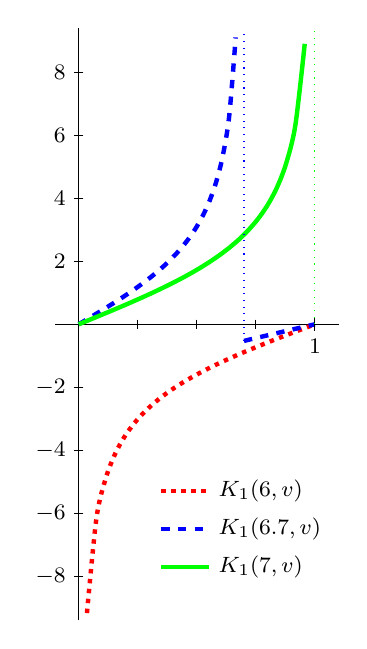
\begin{tikzpicture}[xscale=3.0,yscale=0.4]  % mu = 1, x = 6, 6.7, 7
\footnotesize
%\scriptsize
%\tiny
%\draw[thin,->] (-0.05,0) -- (1.2,0) node[below]{$v$};
\draw[thin] (-0.10,0) -- (1.1,0);
\draw[thin] (0,-9.4) -- (0,9.4);
\draw[red, dotted, ultra thick] % x = 6.0
  plot[domain=0.035:1.0, variable=\v, smooth] 
  (\v, {\v*(6*6-\v*\v)^(1.0-1.5) 
    - (2-\v)*(6*6-(2-\v)*(2-\v))^(1.0-1.5) 
    + (\v+2)*(6*6-(\v+2)*(\v+2))^(1.0-1.5)
    - (4-\v)*(6*6-(4-\v)*(4-\v))^(1.0-1.5)
    + (\v+4)*(6*6-(\v+4)*(\v+4))^(1.0-1.5)
    - (6-\v)*(6*6-(6-\v)*(6-\v))^(1.0-1.5)});
\draw[blue, dashed, ultra thick] % x = 6.7
  plot[domain=0:0.665, variable=\v, smooth] 
  (\v, {\v*(6.7*6.7-\v*\v)^(1.0-1.5) 
    - (2-\v)*(6.7*6.7-(2-\v)*(2-\v))^(1.0-1.5) 
    + (\v+2)*(6.7*6.7-(\v+2)*(\v+2))^(1.0-1.5)
    - (4-\v)*(6.7*6.7-(4-\v)*(4-\v))^(1.0-1.5)
    + (\v+4)*(6.7*6.7-(\v+4)*(\v+4))^(1.0-1.5)
    - (6-\v)*(6.7*6.7-(6-\v)*(6-\v))^(1.0-1.5)
    + (\v+6)*(6.7*6.7-(\v+6)*(\v+6))^(1.0-1.5)});
\draw[blue, dashed, ultra thick] % x = 6.7
  plot[domain=0.70:1, variable=\v, smooth] 
  (\v, {\v*(6.7*6.7-\v*\v)^(1.0-1.5) 
    - (2-\v)*(6.7*6.7-(2-\v)*(2-\v))^(1.0-1.5) 
    + (\v+2)*(6.7*6.7-(\v+2)*(\v+2))^(1.0-1.5)
    - (4-\v)*(6.7*6.7-(4-\v)*(4-\v))^(1.0-1.5)
    + (\v+4)*(6.7*6.7-(\v+4)*(\v+4))^(1.0-1.5)
    - (6-\v)*(6.7*6.7-(6-\v)*(6-\v))^(1.0-1.5)});
\draw[green, ultra thick] % x = 7
  plot[domain=0:0.957, variable=\v, smooth] 
  (\v, {\v*(7*7-\v*\v)^(1.0-1.5) 
    - (2-\v)*(7*7-(2-\v)*(2-\v))^(1.0-1.5) 
    + (\v+2)*(7*7-(\v+2)*(\v+2))^(1.0-1.5)
    - (4-\v)*(7*7-(4-\v)*(4-\v))^(1.0-1.5)
    + (\v+4)*(7*7-(\v+4)*(\v+4))^(1.0-1.5)
    - (6-\v)*(7*7-(6-\v)*(6-\v))^(1.0-1.5)
    + (\v+6)*(7*7-(\v+6)*(\v+6))^(1.0-1.5)});
\draw (1.0,0.2) -- (1.0,-0.2) node[below]{$1$};
\draw[dotted, blue] (0.7,{0.7*(6.7*6.7-0.7*0.7)^(1.0-1.5) 
    - (2-0.7)*(6.7*6.7-(2-0.7)*(2-0.7))^(1.0-1.5) 
    + (0.7+2)*(6.7*6.7-(0.7+2)*(0.7+2))^(1.0-1.5)
    - (4-0.7)*(6.7*6.7-(4-0.7)*(4-0.7))^(1.0-1.5)
    + (0.7+4)*(6.7*6.7-(0.7+4)*(0.7+4))^(1.0-1.5)
    - (6-0.7)*(6.7*6.7-(6-0.7)*(6-0.7))^(1.0-1.5)}) -- (0.7,9.3); % As\'intota
\draw[dotted, green] (1.0,0) -- (1.0,9.3); % As\'intota
\draw[red, dotted, ultra thick] (0.35,-5.3) -- (0.55,-5.3)  node[black, right] {$K_{1}(6,v)$};
\draw[blue, dashed, ultra thick] (0.35,-6.5) -- (0.55,-6.5)  node[black, right] {$K_{1}(6.7,v)$};
\draw[green, ultra thick] (0.35,-7.7) -- (0.55,-7.7)  node[black, right] {$K_{1}(7,v)$};
\draw (0.25,0.15) -- (0.25,-0.15); % node[below]{\scriptsize $0.25$};
\draw (0.5,0.15) -- (0.5,-0.15); % node[below]{\scriptsize $0.5$};
\draw (0.75,0.15) -- (0.75,-0.15); % node[below]{\scriptsize $0.75$};
\draw (0.02,2) -- (-0.02,2) node[left]{$2$};
\draw (0.02,4) -- (-0.02,4) node[left]{$4$};
\draw (0.02,6) -- (-0.02,6) node[left]{$6$};
\draw (0.02,8) -- (-0.02,8) node[left]{$8$};
\draw (0.02,-2) -- (-0.02,-2) node[left]{$-2$};
\draw (0.02,-4) -- (-0.02,-4) node[left]{$-4$};
\draw (0.02,-6) -- (-0.02,-6) node[left]{$-6$};
\draw (0.02,-8) -- (-0.02,-8) node[left]{$-8$};
\end{tikzpicture}
\qquad
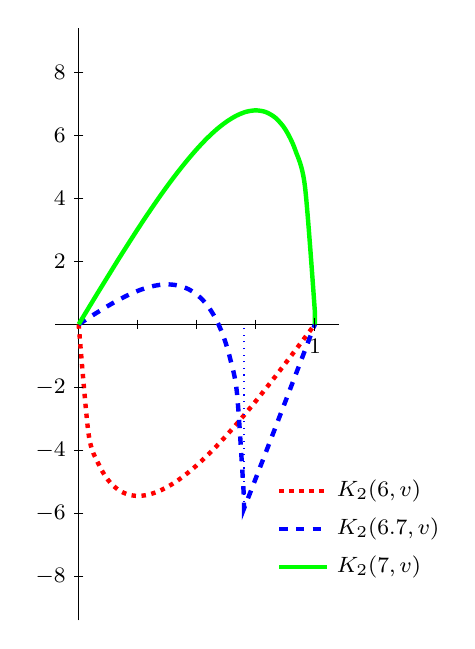
\begin{tikzpicture}[xscale=3.0,yscale=0.4]  % mu = 2, x = 6, 6.7, 7
\footnotesize
%\scriptsize
%\tiny
%\draw[thin,->] (-0.05,0) -- (1.2,0) node[below]{$v$};
\draw[thin] (-0.10,0) -- (1.1,0);
\draw[thin] (0,-9.4) -- (0,9.4);
\draw[red, dotted, ultra thick] % x = 6.0
  plot[domain=0.0:1.0, variable=\v, smooth] 
  (\v, {\v*(6*6-\v*\v)^(2.0-1.5) 
    - (2-\v)*(6*6-(2-\v)*(2-\v))^(2.0-1.5) 
    + (\v+2)*(6*6-(\v+2)*(\v+2))^(2.0-1.5)
    - (4-\v)*(6*6-(4-\v)*(4-\v))^(2.0-1.5)
    + (\v+4)*(6*6-(\v+4)*(\v+4))^(2.0-1.5)
    - (6-\v)*(6*6-(6-\v)*(6-\v))^(2.0-1.5)});
\draw[blue, dashed, ultra thick] % x = 6.7
  plot[domain=0:0.70, variable=\v, smooth] 
  (\v, {\v*(6.7*6.7-\v*\v)^(2.0-1.5) 
    - (2-\v)*(6.7*6.7-(2-\v)*(2-\v))^(2.0-1.5) 
    + (\v+2)*(6.7*6.7-(\v+2)*(\v+2))^(2.0-1.5)
    - (4-\v)*(6.7*6.7-(4-\v)*(4-\v))^(2.0-1.5)
    + (\v+4)*(6.7*6.7-(\v+4)*(\v+4))^(2.0-1.5)
    - (6-\v)*(6.7*6.7-(6-\v)*(6-\v))^(2.0-1.5)
    + (\v+6)*(6.7*6.7-(\v+6)*(\v+6))^(2.0-1.5)}) % ;
%\draw[blue, dashed, ultra thick] % x = 6.7
  --
  plot[domain=0.70:1, variable=\v, smooth] 
  (\v, {\v*(6.7*6.7-\v*\v)^(2.0-1.5) 
    - (2-\v)*(6.7*6.7-(2-\v)*(2-\v))^(2.0-1.5) 
    + (\v+2)*(6.7*6.7-(\v+2)*(\v+2))^(2.0-1.5)
    - (4-\v)*(6.7*6.7-(4-\v)*(4-\v))^(2.0-1.5)
    + (\v+4)*(6.7*6.7-(\v+4)*(\v+4))^(2.0-1.5)
    - (6-\v)*(6.7*6.7-(6-\v)*(6-\v))^(2.0-1.5)});
\draw[green, ultra thick] % x = 7
  plot[domain=0:1.0, variable=\v, smooth] 
  (\v, {\v*(7*7-\v*\v)^(2.0-1.5) 
    - (2-\v)*(7*7-(2-\v)*(2-\v))^(2.0-1.5) 
    + (\v+2)*(7*7-(\v+2)*(\v+2))^(2.0-1.5)
    - (4-\v)*(7*7-(4-\v)*(4-\v))^(2.0-1.5)
    + (\v+4)*(7*7-(\v+4)*(\v+4))^(2.0-1.5)
    - (6-\v)*(7*7-(6-\v)*(6-\v))^(2.0-1.5)
    + (\v+6)*(7*7-(\v+6)*(\v+6))^(2.0-1.5)}) -- (1,0);
\draw (1.0,0.2) -- (1.0,-0.2) node[below]{$1$};
\draw[dotted, blue] (0.7,{0.7*(6.7*6.7-0.7*0.7)^(2.0-1.5) 
    - (2-0.7)*(6.7*6.7-(2-0.7)*(2-0.7))^(2.0-1.5) 
    + (0.7+2)*(6.7*6.7-(0.7+2)*(0.7+2))^(2.0-1.5)
    - (4-0.7)*(6.7*6.7-(4-0.7)*(4-0.7))^(2.0-1.5)
    + (0.7+4)*(6.7*6.7-(0.7+4)*(0.7+4))^(2.0-1.5)
    - (6-0.7)*(6.7*6.7-(6-0.7)*(6-0.7))^(2.0-1.5)}) -- (0.7,0); % Pico
\draw[red, dotted, ultra thick] (0.85,-5.3) -- (1.05,-5.3)  node[black, right] {$K_{2}(6,v)$};
\draw[blue, dashed, ultra thick] (0.85,-6.5) -- (1.05,-6.5)  node[black, right] {$K_{2}(6.7,v)$};
\draw[green, ultra thick] (0.85,-7.7) -- (1.05,-7.7)  node[black, right] {$K_{2}(7,v)$};
\draw (0.25,0.15) -- (0.25,-0.15); % node[below]{\scriptsize $0.25$};
\draw (0.5,0.15) -- (0.5,-0.15); % node[below]{\scriptsize $0.5$};
\draw (0.75,0.15) -- (0.75,-0.15); % node[below]{\scriptsize $0.75$};
\draw (0.02,2) -- (-0.02,2) node[left]{$2$};
\draw (0.02,4) -- (-0.02,4) node[left]{$4$};
\draw (0.02,6) -- (-0.02,6) node[left]{$6$};
\draw (0.02,8) -- (-0.02,8) node[left]{$8$};
\draw (0.02,-2) -- (-0.02,-2) node[left]{$-2$};
\draw (0.02,-4) -- (-0.02,-4) node[left]{$-4$};
\draw (0.02,-6) -- (-0.02,-6) node[left]{$-6$};
\draw (0.02,-8) -- (-0.02,-8) node[left]{$-8$};
\end{tikzpicture}
%---
\caption{The kernels $K_1(x,v)$ and $K_2(x,v)$, $v \in (0,1)$, for $x=6$, $x=6.7$, and $x=7$.}
\label{fig:kernels}
\end{figure}
%-------
% FIN DIBUJOS KERNEL
%-------


The kernel $K_\mu$ allows us to write the function $U_{\mu,1/2}^{\aA}$, $\mu>1/2$, in terms of the function $vU_{1/2,1/2}^\aA(v)$, $v\in[0,1]$.

%---
\begin{Lem}
\label{lem:pp1}
If $\mu>1/2$, then
\[
   U_{\mu,1/2}^{\aA}(x) = \frac{4\Gamma(\mu+1)}{\sqrt{\pi}\,\Gamma(\mu-1/2)x^{2\mu}}
   \int_0^1 vU_{1/2,1/2}^\aA(v)K_\mu(x,v)\,dv.
\]
\end{Lem}

%---
\begin{proof}
What follows is a variant of \cite[\S\,15.2, p.~478]{Wat}.
Using the Sonine-type formula \eqref{eq:sonin-U} for $\eta=1/2$ (that is why we assume that $\mu> 1/2$) we get
\begin{align*}
   U_{\mu,1/2}^{\aA}(x)
   &= \frac{4\Gamma(\mu+1)}{\sqrt{\pi}\,\Gamma(\mu-1/2)}
   \int_0^1 U_{1/2,1/2}^{\aA}(xs) s^{2}(1-s^2)^{\mu-3/2}\,ds
   \\
   &= \frac{4\Gamma(\mu+1)}{\sqrt{\pi}\,\Gamma(\mu-1/2)x^{2\mu}}
   \int_0^x uU_{1/2,1/2}^{\aA}(u) u(x^2-u^2)^{\mu-3/2}\,du.
\end{align*}
Notice that the function
\[
   uU_{1/2,1/2}^{\aA}(u) = \frac{\sqrt{2}\,\Gamma(3/2)}{\sqrt{u}}
   \sum_{m\ge 1} \frac{a_m}{(m\pi)^{1/2}}J_{1/2}(m\pi u)
   = \sum_{m\ge 1}\frac{a_m}{m\pi}\sin(m\pi u)
\]
is odd and periodic with period equal to~$2$.

Assume now that $k\le x< k+1$ and write
\begin{align*}
   &\int_0^x uU_{1/2,1/2}^{\aA}(u)u(x^2-u^2)^{\mu-3/2}\,du
   \\
   &\qquad= \sum_{r=1}^k\int_{r-1}^ruU_{1/2,1/2}^{\aA}(u) u(x^2-u^2)^{\mu-3/2}\,du
   + \int_k^xuU_{1/2,1/2}^{\aA}(u)u(x^2-u^2)^{\mu-3/2}\,du.
\end{align*}
For odd values of $r$ we do the change of variable $v= r-1+u$ in the corresponding integral, while for even values of $r$ we change $v=r-u$. In the last integral, if $k$ is even we do the change of variable $v=k+u$, while if $k$ is odd we change $v=k+1-u$.
The lemma now follows taking into account that the function $uU_{1/2,1/2}^{\aA}(u)$ has period $2$ and is an odd function.
\end{proof}

From now on, given a function $g$, $g(c^-)$ and $g(c^+)$ stand for $\lim_{v\to c^-} g(v)$ and $\lim_{v\to c^+} g(v)$. For the benefit of the reader, we split up the proof of Theorem~\ref{theo:U1/2} into several lemmas.

%---
\begin{Lem}
\label{lem:signoh}
Fix $\mu \in \RR$, $k \in \NN$, and let $h_{\mu,k}(u) = u(k^2 - u^2)^{\mu - 3/2}$ for $u \in [0,k)$. Let $n$ be a nonnegative integer.
\begin{enumerate}
\item[(a)] If $n < \mu - 3/2$, then $h_{\mu,k}^{(n)}(k^-) = 0$.
\item[(b)] If $\mu - 1/2 \notin \NN$ and $\mu - 3/2 \leq n$, then
$
   \sign h_{\mu,k}^{(n)}(k^-)
   = \sign (-1)^n \prod_{j=1}^n (\mu - \tfrac{1}{2} - j).
$
\item[(c)] If $\mu - 1/2 \in \NN$ and $\mu - 3/2 \leq n \leq 2\mu - 2$, then
$
   \sign h_{\mu,k}^{(n)}(k^-)
   = (-1)^{\mu - {3}/{2}}.
$
\item[(d)] If $\mu - 1/2 \in \NN$ and $2\mu - 2 < n$, then $h_{\mu,k}^{(n)}(k^-) = 0$.
\end{enumerate}
\end{Lem}

%---
\begin{proof}
Part (a) is immediate from Leibniz rule for the $n$-th derivative of a product. Part (d) is also immediate, since $h_{\mu,k}$ is in this case a polynomial of degree $2\mu - 2$. Part (b) follows from
% the formula
\[
   h_{\mu,k}^{(n)}(u) = (k^2 - u^2)^{\mu - 3/2 - n}
   \bigg(
   (-1)^n 2^n u^{n+1} \prod_{j=1}^n (\mu - \tfrac{1}{2} - j)
   + (k^2 - u^2) \varphi_n(u)
   \bigg),
\]
where $\varphi_n(u)$ is a polynomial of degree at most $n-1$; this formula is easily proved by induction on~$n$. For the proof of part (c), let us write
$
   h_{\mu,k}(u) = P(u) (k-u)^{\mu - 3/2},
$
where $P(u) = u (k+u)^{\mu - 3/2}$ is a polynomial of degree $\mu - 1/2$ and positive coefficients. Thus, $P^{(j)}(k) > 0$ for $j=0,1,\dots,\mu-1/2$ and
\[
   h_{\mu,k}(u) = (k-u)^{\mu - 3/2}
   \sum_{j=0}^{\mu - 1/2} \frac{P^{(j)}(k)}{j!} (u-k)^j
   = (-1)^{\mu - 3/2}
   \sum_{j=0}^{\mu - 1/2} \frac{P^{(j)}(k)}{j!} (u-k)^{j+\mu-3/2},
\]
which gives the result.
\end{proof}

As a consequence, we have the following:

%---
\begin{Cor}
\label{cor:signoh}
Let $\mu > 1/2$ and let $m$ the integer given by $1/2 + m < \mu \leq 3/2 + m$. Let $n$ be a nonnegative integer. If $n < m$, then
$
   h_{\mu,k}^{(n)}(k^-) = 0;
$
if $m \leq n \leq 2m+1$, then
$
   \sign h_{\mu,k}^{(n)}(k^-) = (-1)^m.
$
\end{Cor}

%---
\begin{proof}
The case $n < m$ follows from part (a) of Lemma~\ref{lem:signoh}, while the case $m \leq n \leq 2m+1$ follows from parts (b) and~(c).
\end{proof}

It might be worthwhile highlighting that $h_{\mu,k}^{2m+1}(u)$ is a product of a Gegenbauer polynomial of parameter $\mu-2m-2 \leq -1/2$ and a nonvanishing function. This follows from Rodrigues formula (see \cite[(4.3.1), p.~67]{Sz}). The proof of our next lemma is essentially a proof that these polynomials have no zeros on the interval $(-1,1)$.

%---
\begin{Lem}
\label{lem:claim1}
Let $\mu > 1/2$ and let $m$ the integer given by $1/2 + m < \mu \leq 3/2 + m$. Then, $h_{\mu,k}^{(2m)}(u)$ is increasing and positive for $u \in [0,k)$ if $m$ is even, and decreasing and negative if $m$ is odd.
\end{Lem}

%---
\begin{proof}
Since
$
   \frac{d}{du} (k^2-u^2)^{\mu-1/2} = -2 (\mu-\frac{1}{2}) h_{\mu,k}(u),
$
Leibniz rule for the derivative of a product gives
\[
   h_{\mu,k}^{2m+1}(u) = -\frac{1}{2(\mu-\frac{1}{2})} \sum_{j=0}^{2m+2}
   \binom{2m+2}{j}
   \frac{d^j}{du^j} \big( (k-u)^{\mu-\frac{1}{2}} \big)
   \frac{d^{2m+2-j}}{du^{2m+2-j}} \big( (k+u)^{\mu-\frac{1}{2}} \big).
\]
Each one of the derivatives on the right-hand side has a constant sign (depending on~$j$) on $(0,k)$ which is easy to determine, so one can deduce that every term in that sum either is $0$ (this only occurs if $\mu = 3/2 + m$) or has sign $(-1)^{m+1}$. This proves that
$
   \sign h_{\mu,k}^{2m+1}(u) = (-1)^m
$
in $(0,k)$. That is, $h_{\mu,k}^{(2m)}(u)$ is increasing if $m$ is even, and decreasing if $m$ is odd. To finish the proof, just observe that $h_{\mu,k}$ is an odd function, so $h_{\mu,k}^{(2m)}$ is odd as well, and $h_{\mu,k}^{(2m)}(0) = 0$.
\end{proof}

%---
\begin{Lem}
\label{lem:claim2}
Let $\mu > 1/2$ and $m$ the integer given by $1/2 + m < \mu \leq 3/2 + m$. Let $j$ be an integer such that $m \leq 2j \leq 2m$.
\begin{enumerate}
\item[(a)] If $k$ is odd and large enough, then $\sign \frac{d^{2j+1}}{dv^{2j+1}}K_\mu(k,0) = (-1)^m$.
\item[(b)] If $k$ is even and large enough, then $\sign \frac{d^{2j+1}}{dv^{2j+1}}K_\mu(k,1) = (-1)^m$.
\end{enumerate}
\end{Lem}

%---
\begin{proof}
Assume that $k$ is odd.
It follows from~\eqref{def:kerimpar} that
\begin{equation}
\label{eq:kmukv}
   K_\mu(k,v) = \sum\limits_{r=1}^{(k+1)/2} h_{\mu,k} (2r-2+v)
   - \sum\limits_{r=1}^{(k-1)/2} h_{\mu,k} (2r-v).
\end{equation}
Now,
$
   h_{\mu,k}(u) =
   k^{2\mu-2} h_{\mu,1}(\tfrac{u}{k}).
$
Hence,
$
   h_{\mu,k}^{(2j+1)}(u) = k^{2\mu - 2j - 3} h_{\mu,1}^{(2j+1)}(\tfrac{u}{k})
$
and \eqref{eq:kmukv} gives
\begin{align*}
   \frac{d^{2j+1}}{dv^{2j+1}} K_\mu(k,0)
   &= h_{\mu,k}^{(2j+1)}(0) + \sum_{r=1}^{(k-1)/2} 2 h_{\mu,k}^{(2j+1)}(2r)
   \\
   &= k^{2\mu-2j-3} h_{\mu,1}^{(2j+1)}(0)
   + k^{2\mu-2j-3} \sum_{r=1}^{(k-1)/2} 2 h_{\mu,1}^{(2j+1)}(\tfrac{2}{k}r),
\end{align*}
so
\[
   k^{-2\mu + 2j +2} \frac{d^{2j+1}}{dv^{2j+1}} K_\mu(k,0)
   = k^{-1} h_{\mu,1}^{(2j+1)}(0)
   + \sum_{r=1}^{(k-1)/2} \tfrac{2}{k} h_{\mu,1}^{(2j+1)}(\tfrac{2}{k} r).
\]
The last term is a Riemann sum of the integral of $h_{\mu,1}^{(2j+1)}$ on the interval $(0,1)$. Therefore,
\[
   \lim_{k \to +\infty} k^{-2\mu + 2j +2} \frac{d^{2j+1}}{dv^{2j+1}} K_\mu(k,0)
   = \int_0^1 h_{\mu,1}^{(2j+1)}(u) \, du
   = h_{\mu,1}^{(2j)}(1^-),
\]
taking into account that $h_{\mu,1}(u)$ is an odd function, so $h_{\mu,1}^{(2j)}(0) = 0$. This, together with Corollary~\ref{cor:signoh}, proves~(a).

If $k$ is even, the same arguments give
$
   k^{-2\mu + 2j +2} \frac{d^{2j+1}}{dv^{2j+1}} K_\mu(k,1)
   = \sum_{r=1}^{k/2} \frac{2}{k} h_{\mu,1}^{(2j+1)}(\frac{2r-1}{k}),
$
which is again a Riemann sum of the integral of $h_{\mu,1}^{(2j+1)}$ on the interval $(0,1)$.
\end{proof}

Before going on, we remark the following elementary properties of convex functions. Let $g : [0,1) \to \RR$ be a twice differentiable function such that $g(0) = 0$ and $g''(v) > 0$ for $v \in (0,1)$.
\begin{enumerate}
\item[(a)] If $g(1^-) = 0$, then $g(v) < 0$ for every $v \in (0,1)$.
\item[(b)] If $g'(0) > 0$, then $g(v) > 0$ for every $v \in (0,1)$.
\end{enumerate}
Let us state also the symmetric situation, for further reference. Let $g : (0,1] \to \RR$ be a twice differentiable function such that $g(1) = 0$ and $g''(v) > 0$ for every $v \in (0,1)$.
\begin{enumerate}
\item[(a)] If $g(0^+) = 0$, then $g(v) < 0$ for every $v \in (0,1)$.
\item[(b)] If $g'(1) < 0$, then $g(v) > 0$ for every $v \in (0,1)$.
\end{enumerate}

We can now prove that, for any $\mu > 1/2$, the kernel $K_{\mu}(k,v)$ has constant sign for $v \in (0,1)$ if $k \in \NN$ is big enough (depending on~$\mu$).

%---
\begin{Lem}
\label{lem:pp2}
Let $\mu > 1/2$ and let $m$ the integer given by $1/2 + m < \mu \leq 3/2 + m$.
Then, there exists some $k_\mu\in\NN$ such that for any integer $k\ge k_\mu$,
\[
   \sign K_{\mu}(k,v) = (-1)^{\lfloor m/2\rfloor+k+1},\quad v\in(0,1).
\]
More precisely, for $1/2 < \mu \leq 5/2$, we can take $k_\mu=1$.
\end{Lem}

%---
\begin{proof}
From~\eqref{def:kerpar} and~\eqref{def:kerimpar}, it follows that
\begin{equation}
\label{eq:llor}
   K_\mu(k,v) = \begin{cases}
   \sum\limits_{r=1}^{k/2}(h_{\mu,k} (2r-2+v)-h_{\mu,k} (2r-v)),
   &\text{for } k \text{ even},
   \\[8pt]
   \sum\limits_{r=1}^{(k+1)/2}h_{\mu,k} (2r-2+v) - \sum\limits_{r=1}^{(k-1)/2}h_{\mu,k} (2r-v),
   &\text{for } k \text{ odd}.
\end{cases}
\end{equation}
If $1/2 < \mu\le 3/2$, then for any $k \in \NN$ the function $h_{\mu,k}(u)$ is increasing and positive, so that \eqref{eq:llor} gives easily that
\[
   \sign K_{\mu}(k,v) = (-1)^{k+1}, \quad v \in(0,1).
\]
This proves the lemma for $1/2 < \mu \leq 3/2$.

Assume now that $1/2 + m < \mu \leq 3/2 + m$, with $m \geq 1$. The same argument, together with Lemma~\ref{lem:claim1}, proves that
\[
   \sign \frac{d^{2m}}{dv^{2m}} K_\mu(k,v) = (-1)^{k+1+m},
   \quad v \in (0,1).
\]
Let us take
\[
   g_j(v) = (-1)^{k+1+m} \frac{d^{2j}}{dv^{2j}} K_\mu(k,v),
\]
for $m \leq 2j \leq 2m$. We have just proved that $g_m(v) > 0$ on $(0,1)$.

If $m=1$ we can skip the following iteration, which is the only step where $k$ is required to be large enough. If $m \geq 2$, let us suppose that $m \leq 2j \leq 2m-2$ and $g_{j+1}(v) > 0$ on $(0,1)$. Then, $g_j''(v) = g_{j+1}(v) > 0$ on $(0,1)$. If $k$ is odd,
\[
   g_j(0) = (-1)^{k+1+m} \frac{d^{2j}}{dv^{2j}} K_\mu(k,0)
   = (-1)^{k+1+m} h_{\mu,k}^{(2j)}(0)
   = 0
\]
and
\[
   g_j'(0) = (-1)^{k+1+m} \frac{d^{2j+1}}{dv^{2j+1}} K_\mu(k,0)
   > 0
\]
for $k$ large enough, by Lemma~\ref{lem:claim2}. By convexity, $g_j(v) > 0$ on $(0,1)$. If $k$ is even, $g_j(1) = 0$ and $g_j'(1) < 0$, so again $g_j(v) > 0$ on $(0,1)$. As a result of this iteration we conclude that
\[
   (-1)^{k+1+m} \frac{d^{2j}}{dv^{2j}} K_\mu(k,v)
   > 0
\]
on $(0,1)$, for $j = \lfloor(m+1)/2\rfloor$. Now, let us take
\[
   f_j(v) = (-1)^{k+1+m+\lfloor(m+1)/2\rfloor-j} \frac{d^{2j}}{dv^{2j}} K_\mu(k,v).
\]
For $j = \lfloor(m+1)/2\rfloor$ we have just proved that $f_j(v) > 0$ on $(0,1)$. Let us iterate again: suppose that $0 \leq j < \lfloor(m+1)/2\rfloor$ and $f_{j+1}(v) > 0$ on $(0,1)$. Then, $(-f_j)''(v) = f_{j+1}(v) > 0$ on $(0,1)$. If $k$ is odd,
\[
   -f_j(0) = (-1)^{k+m+\lfloor(m+1)/2\rfloor-j} h_{\mu,k}^{(2j)}(0)
   = 0
\]
and
\[
   -f_j(1^-) = (-1)^{k+m+\lfloor(m+1)/2\rfloor-j} h_{\mu,k}^{(2j)}(k^-)
   = 0,
\]
by Corollary~\ref{cor:signoh}. By convexity, $f_j(v) > 0$ on $(0,1)$. If $k$ is even, $f_j(1) = 0$ and $f_j(0^+) = 0$, so again $f_j(v) > 0$ on $(0,1)$.

As a result of this second iteration, we conclude that
\[
   (-1)^{k+1+m+\lfloor(m+1)/2\rfloor} K_\mu(k,v) > 0
\]
on $(0,1)$, that is,
\[
   \sign K_\mu(k,v) = (-1)^{k+1+m+\lfloor(m+1)/2\rfloor}
   = (-1)^{\lfloor m/2\rfloor + k+1}.
   \qedhere
\]
\end{proof}

%---
\begin{proof}[Proof of Theorem~\ref{theo:U1/2}]
It is now an easy consequence of Lemmas~\ref{lem:pp1} and~\ref{lem:pp2}.
\end{proof}

%---
\begin{Cor}
\label{cor:U1/2}
Let $-1/2<\mu\le 1/2$. Assume that the function
\[
   vU_{1/2,1/2}^{\aA}(v) = \sum_{m\ge 1} \frac{a_m}{m\pi}\sin(m\pi v), \quad v\in [0,1],
\]
has constant sign on $(0,1)$ and
\begin{equation}
\label{eq:U1-v}
   \frac{vU_{1/2,1/2}^{\aA}(v)}{1-v} \text{ is bounded on a neighbourhood of $v=1$}.
\end{equation}
Then the function $U_{\mu,1/2}^{\aA}$ has at least one zero on each interval $[k,k+1)$, $k\ge 0$.
\end{Cor}

%---
\begin{proof}
Using the Sonine formula \eqref{eq:sonin-U} for $\eta=-1/2$, we get
\begin{equation}
\label{eq:sonin-a}
   U_{\mu,1/2}^{\aA}(x) = \frac{2\Gamma(\mu +1)}{\sqrt{\pi}\,\Gamma(\mu+1/2)}
   \int_0^1U_{-1/2,1/2}^{\aA}(xs) (1-s^2)^{\mu-1/2} \,ds.
\end{equation}
Notice that
\begin{equation}
\label{eq:derU}
   (uU_{1/2,1/2}^{\aA})'(u) = U_{-1/2,1/2}^{\aA}(u).
\end{equation}
So, integrating by parts in \eqref{eq:sonin-a}, we get
\begin{align}
\label{eq:Ulim}
   U_{\mu,1/2}^{\aA}(x) = \frac{2\Gamma(\mu +1)}{\sqrt{\pi}\,\Gamma(\mu+1/2)}
   & \Big( \lim_{s\to 1^-}sU_{1/2,1/2}^{\aA}(sx)(1-s^2)^{\mu-1/2}
   \\
\nonumber
   &\quad + 2(\mu-1/2)
   \int_0^1 sU_{1/2,1/2}^{\aA}(xs)s(1-s^2)^{\mu-3/2}\,ds\Big).
\end{align}
Since the function $U_{1/2,1/2}^{\aA}(v)$ is continuous at $v=0$, and $vU_{1/2,1/2}^{\aA}(v)$ has period $2$ and is an odd function, we deduce for $k$ even and positive that
\begin{equation}
\label{eq:U1-s}
   \frac{sU_{1/2,1/2}^{\aA}(sk)}{1-s} \text{ is bounded on a neighbourhood of }s=1,
\end{equation}
because
\[
   \frac{s U_{1/2,1/2}^{\aA}(sk)}{1-s}
   = \frac{ks U_{1/2,1/2}^{\aA}(s k)}{k(1-s)}
   = \frac{(ks-k) U_{1/2,1/2}^{\aA}(s k-k)}{k(1-s)}
   = -U_{1/2,1/2}^{\aA}(sk-k).
\]
But \eqref{eq:U1-s} is still true for $k$ odd, as can be easily deduced using
\eqref{eq:U1-v} and, again, that the function $vU_{1/2,1/2}^{\aA}(v)$ has period $2$ and is odd,
because
\[
   \frac{s U_{1/2,1/2}^{\aA}(s k)}{1-s} = \frac{ks U_{1/2,1/2}^{\aA}(sk)}{k(1-s)}
   = \frac{(k s-k+1) U_{1/2,1/2}^{\aA}(sk-k+1)}{k(1-s)}
   = \frac{v U_{1/2,1/2}^{\aA}(v)}{1-v}
\]
with $v=k(s-1)+1$.

Since $-1/2<\mu$, from \eqref{eq:Ulim} and \eqref{eq:U1-s} we have,
for any positive integer~$k$,
\[
   U_{\mu,1/2}^{\aA}(k) = \frac{4\Gamma(\mu +1)}{\sqrt{\pi}\,\Gamma(\mu-1/2)}
   \int_0^1sU_{1/2,1/2}^{\aA}(ks)s(1-s^2)^{\mu-3/2}\,ds.
\]
Proceeding as in Lemma~\ref{lem:pp1}, we write
\[
   U_{\mu,1/2}^{\aA}(k) = \frac{4\Gamma(\mu +1)}{\sqrt{\pi}\,\Gamma(\mu-1/2)k^{2\mu}}
   \int_0^1 vU_{1/2,1/2}^{\aA}(v)K_{\mu}(k,v)\,dv.
\]
Now, for $-1/2< \mu\le 1/2$ the function $h_{\mu,k}(u)$ is increasing in $[0,k)$. Hence, the kernel $K_{\mu}(k,v)$ has constant sign equal to $(-1)^{k+1}$ for $v\in(0,1)$, for every $k\ge 1$.

The function $U_{\mu,1/2}^{\aA}(x)$ has also at least one zero on $[0,1)$. Indeed, assume that $vU_{1/2,1/2}^{\aA}(v)$ is positive in $(0,1)$ (the proof is similar if it is negative). Then, on the one hand, according to the discussion in the previous line the sign of $U_{\mu,1/2}^{\aA}(1)$ is negative. On the other hand, since $vU_{1/2,1/2}^{\aA}(v)$ vanishes at $v=0$, it must be increasing at $v=0$ and so \eqref{eq:derU} gives that $U_{-1/2,1/2}^{\aA}(0)$ is positive. Hence, using \eqref{eq:sonin-a}, we can conclude that $U_{\mu,1/2}^{\aA}(0)$ is positive.
\end{proof}

%----------
\section{Conjectures on the zeros of the functions $U_{\mu,\nu}^\aA$}
\label{sec:zerosU}
%----------

As we pointed out in the Introduction, we guess that Theorem~\ref{theo:U1/2} is also true for $\mu>-1$ without any additional assumption:

%---
\begin{Conjecture}
\label{conj:zeros}
For $\mu>-1$ and $k\in \NN$ big enough (depending on $\mu$), the function $U_{\mu,1/2}^{\aA}$ defined in \eqref{eq:gfs} has at least one zero in each interval $[k,k+1)$.
\end{Conjecture}

It is well-known that the zeros of the Bessel functions $J_\mu$, $\mu>-1$, enjoy a number of interesting properties (see \cite[Ch.~XV]{Wat}). Some of those properties are that the function $J_\mu$ has infinitely many positive zeros, all of them simple; they interlace with the zeros of $J_{\mu +1}$ and the $k$-th zero of $J_\mu$ is an increasing function of~$\mu$.

Except for the fact that the function $U_{\mu,1/2}^\aA$ has infinitely many positive zeros, in general, those properties seem to fail for the zeros of the functions $U_{\mu,1/2}^\aA$, as the following numerical example suggests.
Before going on with it we stress that the computation of zeros of special functions is a difficult task (see, for instance, \cite{GS}), in particular when, as it happens with the function $U_{\mu,1/2}^\aA$, they are defined as infinite series. In the following example and in others in this section, we have chosen sequences $a_m$ for which $a_m=0$, $m\ge 4$. For some other examples in this and in following sections, however, we have made a huge amount of experiments with sequences with much more non-null terms so as to check the behavior described in our conjectures. The use of series with many non-null summands
may also have an influence on the zeros, so we have looked for changes of sign that are heuristically meaningful. More precisely, the values at the endpoints of an interval $[k,k+1]$ (whose change of signs implies the existence of zeros in that interval) should be big enough compared with the estimated bound for the error terms.

Let us go on with our first example. Consider the sequence
$a_1=\frac{1}{3}$, $a_2=0$, $a_3=1$, and $a_m=0$ for $m\ge 4$.
%\[
%   a_1=\frac{1}{3},\quad a_2=0, \quad a_3=1,\quad a_m=0,\ m\ge 4.
%\]
Hence,
\[
   xU_{1/2,1/2}^\aA(x) = \frac{1}{3\pi}(\sin(\pi x)+\sin(3\pi x)).
\]
It is easy to check that $xU_{1/2,1/2}^\aA(x)\ge 0$ for $x\in [0,1]$ and has double zeros at $x=(2k+1)/2$, $k=0,1,2,\dots$
The zeros of $U_{0.4,1/2}^\aA$ do not interlace with the zeros of $U_{1.4,1/2}^\aA$. Indeed, $U_{0.4,1/2}^\aA$ has six zeros on the interval $[0,2]$ but $U_{1.4,1/2}^\aA$ has only one zero on that interval.
On the other hand, the first positive zero of $U_{0.4,1/2}^\aA$ is less than $0.45$ and its second zero is greater than $0.53$; but the first positive zero of $U_{0.48,1/2}^\aA$ is between $0.45$ and $0.5$ and its second zero lies between $0.5$ and $0.53$. This shows that the second zero of $U_{\mu,1/2}^\aA$ is not an increasing function of~$\mu$.

The interlacing property of the zeros of $J_\mu$ and $J_{\mu +1}$ follows from the identities
\[
   (x^{\mu+1}J_{\mu+1}(x))' = x^{\mu+1}J_\mu(x),
   \qquad
   (x^{-\mu}J_{\mu}(x))' = -x^{-\mu}J_{\mu+1}(x).
\]
These identities give the following ones for the functions $U_{\mu,\nu}^\aA$:
\begin{align}
\label{eq:derps1}
   (x^{2\mu+2}U_{\mu+1,\nu}^\aA (x))' &= 2(\mu+1)x^{2\mu+1}U_{\mu,\nu}^\aA (x),
   \\
\label{eq:derps2}
   (U_{\mu,\nu}^{\tilde \aA}(x))' &= -\frac{xU_{\mu+1,\nu}^\aA(x)}{2(\mu+1)},
\end{align}
where $\tilde \aA=(a_m/j_{m,\nu}^2)_m$.

The change of the sequence $\aA$ in the identity \eqref{eq:derps2} does not allow to proceed like with the Bessel functions.
But \eqref{eq:derps1} can be used to show that $U_{\mu,1/2}^\aA$ has zeros at each interval $[k,k+2)$, if $-1< \mu <- 1/2$.

Our Conjecture~\ref{conj:onezero} establishes that under the assumption that the function $vU_{1/2,1/2}^\aA(v)$ has constant sign on $[0,1]$ (see Theorem~\ref{theo:U1/2}), the zeros of the function $U_{\mu,1/2}^\aA$ seem to behave more regularly if $\mu$ is big enough. We have a lot of computational evidences for Conjecture~\ref{conj:onezero}. This evidences also show that the threshold value $\mu_0$ from which this conjecture would hold could be a relatively small number such as~$12$.

When $vU_{1/2,1/2}^{\aA}(v)$ changes its sign in $(0,1)$, the quantification of the number of zeros of the function $U_{\mu,1/2}^{\aA}$ on an interval $[k,k+1)$ in Theorem~\ref{theo:U1/2} seems to depend not on the number of changes of sign of $xU_{1/2,1/2}^{\aA}(x)$ in $(0,1)$, but on its shape.
We display here three illustrative examples.

\begin{enumerate}
\item Consider the sequence
$a_1 =-\sqrt 2/2$, $a_2=1$, and $a_m=0$ for $m\ge 3$.
%\[
%   a_1 =-\sqrt 2/2,\quad a_2=1,\quad a_m=0,\ m\ge 3.
%\]
Then,
\[
   xU_{1/2,1/2}^{\aA}(x)=\frac{1}{2\pi}(-\sqrt 2\sin(\pi x)+\sin(2\pi x)).
\]
As a consequence, this function has exactly one change of sign on $(0,1)$, at $1/4$.
When $\mu$ is small, say $0.55$, the function
$U_{\mu,1/2}^{\aA}$ seems to have three zeros in each interval $[2k+1,2k+2)$ and one zero in each interval $[2k,2k+1)$, for $k\ge 1$. However, when $\mu$ increases ($\mu\ge 1$ is enough), the function $U_{\mu,1/2}^{\aA}$ seems to have just one zero in each interval $[k,k+1)$, for $k$ big enough.

\item Consider the sequence
$a_1=0$, $a_2 =1$, and $a_m=0$ for $m\ge 3$.
%\[
%   a_1=0,\quad a_2 =1,\quad a_m=0,\ m\ge 3.
%\]
Then,
\[
   U_{\mu,1/2}^{\aA}(x) = \frac{\Gamma(\mu+1)}{(\pi x)^\mu}J_\mu (2\pi x).
\]
In particular, $xU_{1/2,1/2}^{\aA}(x)=\sin(2\pi x)/(2\pi)$ for $x\in[0,1]$,
which has exactly one change of sign on $(0,1)$, at $x = 1/2$.
Obviously, the zeros of $U_{\mu,1/2}^{\aA}(x)$
are $j_{m,\mu}/(2\pi)$. Hence, using \cite[\S\,15.35, p.~492]{Wat}, one sees that for $\mu >1$ and $k>(2\mu+1)(2\mu+3)/\pi$, $k\in \NN$, the function $U_{\mu,1/2}^{\aA}(x)$ has two zeros on each interval $[k,k+1)$. So, the number of changes of sign of $xU_{1/2,1/2}^{\aA}(x)$
on $(0,1)$ is the same as in the first example, but now the function $U_{\mu,1/2}^{\aA}$ has always just two zeros on each interval $[k,k+1)$, for $k$ big enough.
\item Consider the sequence
%\[
%   a_m = \begin{cases}
%   -\frac{1-2\sin(3\pi/8)}{3(1-2\sin(\pi/8))}
%   = \frac{1}{3} \left(1+\sqrt{4+4\sqrt{2}}\right), & m=1,
%   \\
%   -\frac{2\sqrt 2(-\sin(\pi/8)+\sin(3\pi/8))}{3(1-2\sin(\pi/8))}
%   = -\frac{2}{3} \left(\sqrt{2}+\sqrt{2+\sqrt{2}}\right), &m=2,
%   \\
%   1, &m=3,
%   \\
%   0, & m\ge 4.
%   \end{cases}
%\]
$a_1 = -\frac{1-2\sin(3\pi/8)}{3(1-2\sin(\pi/8))}$,
$a_2 = -\frac{2\sqrt 2(-\sin(\pi/8)+\sin(3\pi/8))}{3(1-2\sin(\pi/8))}$,
$a_3 = 1$, and $a_m = 1$ for $m\ge 4$;
%\[
%   a_m = \begin{cases}
%   -\frac{1-2\sin(3\pi/8)}{3(1-2\sin(\pi/8))}
%   = \frac{1}{3} \left(1+\sqrt{4+4\sqrt{2}}\right), & m=1,
%   \\
%   -\frac{2\sqrt 2(-\sin(\pi/8)+\sin(3\pi/8))}{3(1-2\sin(\pi/8))}
%   = -\frac{2}{3} \left(\sqrt{2}+\sqrt{2+\sqrt{2}}\right), &m=2,
%   \\
%   1, &m=3,
%   \\
%   0, & m\ge 4.
%   \end{cases}
%\]
notice that $a_1 = \frac{1}{3} \big(1+\sqrt{4+4\sqrt{2}}\big)$
and $a_2 = -\frac{2}{3} \big(\sqrt{2}+\sqrt{2+\sqrt{2}}\big)$.
It is then easy to see that $xU_{1/2,1/2}^{\aA}(x)$ has exactly two changes of sign on $(0,1)$, at $x=1/8$ and $x=1/4$. But, for $\mu > 2$, the function $U_{\mu,1/2}^{\aA}$ seems to have just one zero on each interval $[k,k+1)$ for $k$ big enough.
So, the number of changes of sign of $xU_{1/2,1/2}^{\aA}(x)$
in $(0,1)$ is bigger than in the previous example, but the function $U_{\mu,1/2}^{\aA}$, for $\mu>2$, seems to have less zeros on each interval $[k,k+1)$, for $k$ big enough.
\end{enumerate}

The extension of our conjectures for $\nu\not =1/2$ needs further research.
The computational evidences show that the normalization factor $\pi /j_{1,\nu}$ will probably play an important role. This
is the case of Conjecture~\ref{conj:zeros}, which can be extended as follows.

%---
\begin{Conjecture}
For $\mu,\nu>-1$ and $k\in \NN$ big enough (depending on $\mu$ and $\nu$), the function $U_{\mu,\nu}^{\aA}$ defined in \eqref{eq:gfs} has zeros in each interval $[k\pi /j_{1,\nu},(k+1)\pi /j_{1,\nu})$.
\end{Conjecture}

The case of Conjecture~\ref{conj:onezero} is more obscure: we have not found yet a sound candidate for the function $vU_{1/2,1/2}^{\aA}(v)$, $v\in [0,1]$. On the one hand, we do not find here the periodic structure appearing when $\nu=1/2$. This structure allowed us to find the kernel $K_\mu (x,v)$ and the expression of $U_{\mu,1/2}^{\aA}(x)$ in terms of $vU_{1/2,1/2}^{\aA}(v)$, $v\in [0,1]$ (see Lemma~\ref{lem:pp1} for details). On the other hand, we have not found computational evidence to exclude that the same hypothesis on the constant sign of the function $vU_{1/2,1/2}^{\aA}(v)$ in $[0,1]$ could also work for any $\nu$ as for the case $\nu=1/2$. Hence, extending Conjecture~\ref{conj:onezero} would require a better understanding of this non-periodic situation.


%----------
\section{The functions $V_{\mu,\nu}^b$}
\label{sec:funV}
%----------

In this section, we study the functions $V_{\mu,\nu}^{2n+1}(x)$ defined in \eqref{eq:gfs1} and prove that for $x\in [0,1]$ they are polynomials which can be explicitly computed using a recurrence relation. We need the residue theorem for analytic functions, so it is more convenient to consider the entire functions $\I_\mu$ defined by
\begin{equation}
\label{eq:ial}
  \I_\mu(z) = 2^\mu \Gamma(\mu+1) \frac{J_\mu(iz)}{(iz)^\mu}
  = \Gamma(\mu+1) \sum_{n=0}^\infty \frac{(z/2)^{2n}}{n!\,\Gamma(n+\mu+1)}
\end{equation}
instead of the Bessel functions $J_\mu$, where we now assume $\mu\in \CC\setminus\{-1,-2,\dots \}$.

Given a function $f$ holomorphic in $z=0$ and a complex number $\nu\in \CC\setminus \{-1,-2,\dots\}$, our tool in this section will be the Taylor coefficients $(\dd_n^{f,\nu})_{n\ge 0}$ of $f(z)/\I_{\nu}(iz)$:
\begin{equation}
\label{eq:diarrea}
   \frac{f(z)}{\I_{\nu}(iz)} = \sum_{n=0}^\infty \dd^{f,\nu}_{n} z^n.
\end{equation}
The cases
\[
   f(z) = \I_{\nu-1} (ixz) + \frac{ixz}{2\nu }\I_{\nu} (ixz),
   \qquad
   f(z) = \I_\nu (ixz) + \frac{ixz}{2(\nu +1)}\I_{\nu +1} (ixz),
\]
$x\in \CC$, were studied in \cite{CDPV} and \cite{DPV}, respectively
(some other cases can be found in~\cite{CMV}).

It is known that
$
  \I_{\nu}(iz) = \sum_{n=0}^\infty {(-1)^nz^{2n}}/{\cc_{2n,\nu}},
$
where
\begin{equation}
\label{eq:garr}
   \cc_{n,\nu} = \begin{cases}
   2^{2k}k!\,(\nu+1)_k, & \text{if } n=2k,
   \\
   2^{2k+1}k!\,(\nu+1)_{k+1}, & \text{if }n=2k+1
   \end{cases}
\end{equation}
and $(a)_j$ is the Pochhammer symbol.
Writing $f(z) = \sum_{n=0}^\infty a_nz^n$,
we get for $(\dd_n^{f,\nu})_{n\ge 0}$ the recurrence formulas
\begin{equation}
\label{eq:recus}
\begin{aligned}
   a_{2n}
   &= \dd^{f,\nu}_{2n}+\frac{(-1)^n}{\cc_{2n,\nu}}
   \sum_{j=0}^{n-1} (-1)^k\binom{2n}{2j}_{\!\nu} \, \dd^{f,\nu}_{2j},
\\
   a_{2n+1}
   &= \dd^{f,\nu}_{2n+1}+\frac{(-1)^n}{\cc_{2n+1,\nu}}
   \sum_{j=0}^{n-1} (-1)^k\binom{2n+1}{2j}_{\!\nu} \, \dd^{f,\nu}_{2j+1},
\end{aligned}
\end{equation}
where $\binom{n}{j}_{\!\nu} = \frac{\cc_{n,\nu}}{\cc_{j,\nu}\cc_{n-j,\nu}}$.

%---
\begin{Theo}
\label{theo:tscoj}
Assume that $f$ is an entire function satisfying
\begin{equation}
\label{eq:est}
   |f(z)| \le c(1+|z|)^Ne^{\kappa |\Im z|}, \quad z\in \CC,
\end{equation}
for certain constants $0\le \kappa\le 1$, $c>0$ and $N\in \RR$.
Let $\nu \in \CC\setminus \{-1,-2,\dots \}$ and $n$ a nonnegative integer. Assume that they satisfy
\[
   \Re \nu +N < \begin{cases}
   n-1/2, &\kappa =1,
   \\
   n+1/2, &0\le \kappa<1.
   \end{cases}
\]
Then
\begin{equation}
\label{eq:smargg}
   \frac{d^n}{dz^n} \left(\frac{f(z)}{\I_{\nu}(iz)}\right)
   = \sum_{m\in\ZZO} \frac{2(-1)^{n+1}(\nu+1)n!f(j_m)}{j_m\I_{\nu+1}(ij_m)(z-j_m)^{n+1}},
\end{equation}
which converges uniformly in bounded subsets of~$\CC \setminus \{j_m : m\in \ZZO\}$.
\end{Theo}

%---
\begin{proof}
The proof proceeds as that of Theorem~1.1 ($n=0$) and Corollary~2.1 ($n\ge 1$) of \cite{DPV}, and is based in the estimate
\begin{equation}
\label{eq:cotasxx}
  |J_\nu (w)| \ge c\,\frac{e^{|\Im w|}}{|w|^{1/2}}.
\end{equation}
Take a large circle $D=\{z\in \CC : |z| = A\}$ of radius $A>|z|$ with the only condition, at the moment, that none of the points $j_m$, $m\in \ZZO$, must lie in~$D$, and consider
$\frac{1}{2\pi i} \int_{D} \frac{f(w)}{(w-z)\I_{\nu}(iw)}\, dw$.
The poles of $\frac{f(w)}{(w-z)\I_{\nu}(iw)}$ in $D$, all of them simple, are $z$ and those $j_m \in D$.
Thus, the calculus of residues gives
\begin{equation}
\label{eq:residuo}
   \frac{1}{2\pi i} \int_{\partial D}
   \frac{f(w)}{(w-z)\I_{\nu}(iw)} \, dw
   = \frac{f(z)}{\I_{\nu}(iz)} + \sum_{|j_m| <A}
   \frac{2(\nu+1)f(j_m)}{j_m\I_{\nu+1}(ij_m)(z-j_m)}.
\end{equation}
Using \eqref{eq:cotasxx} and \eqref{eq:est}, we get, for $w\in D$, $\left|\frac{f(w)}{\I_{\nu}(iw)}\right| \le \tilde c\, |w|^{\Re \nu+N+1/2}e^{(\kappa-1)|\Im w|}$.
This gives
\begin{align*}
   \left|
   \frac{1}{2\pi i} \int_{D}
   \frac{f(w)}{(w-z)\I_{\nu}(iw)}\, dw
   \right|
   &\leq \frac{1}{2\pi} \int_{-\pi}^{\pi}
   \frac{A}{A - |z|} \cdot
   \tilde{c} \, A^{\Re \nu+N+1/2}e^{(\kappa-1) |A\sin s| } \, ds.
\end{align*}
Proceeding as in the proof of Theorem~1.1 of \cite{DPV}, we can see that either for $\kappa=1$ and $\Re \nu+N+1/2<0 $ or for $0\le \kappa <1$ and $\Re \nu+N-1/2<0$,
the left-hand side of~\eqref{eq:residuo} goes uniformly to $0$ as $A$ goes to infinity. This proves~\eqref{eq:smargg} for $n = 0$.
For $n\ge 1$, the proof goes as that of Corollary~2.1 of~\cite{DPV}.
\end{proof}

Let us suppose that a function $f$ satisfies the conditions of Theorem~\ref{theo:tscoj}.
Taking $z=0$ in \eqref{eq:smargg} gives
\[
   \dd_n^{f,\nu} = \sum_{m\in\ZZO} \frac{2(\nu+1)f(j_m)}{j_m^{n+2}\I_{\nu+1}(ij_m)}.
\]
The sums
\[
   \sum_{m\in\ZZO} \frac{2(\nu+1)f(j_m)}{j_m^{n+2}\I_{\nu+1}(ij_m)}
\]
inherit then the recurrence relation \eqref{eq:recus} for the numbers $(\dd_n^{f,\nu})_{n\ge 0}$, and can be computed recursively from the Taylor coefficients $\gamma_{n,\nu}$ \eqref{eq:garr} and $a_n$ (of the function~$f$).

We can now compute explicitly the value of the functions $V_{\mu,\nu}^{2n+1}$ defined by~\eqref{eq:gfs1} in $[0,1]$, using the numbers $\dd_n^{\mu,\nu}$ associated to the entire function $f_v(z)=\I_\mu (ivz)$, $v\in[0,1]$. Since $\I_\mu$ is an even function, we have $\dd_{2n+1}^{\mu,\nu}=0$. The numbers $\dd_{2n}^{\mu,\nu}$ can be computed from the recursion~\eqref{eq:recus}; in this case, $a_{2n}=(-1)^nv^n/\gamma_{2n,\mu}$. The first numbers are
\begin{align*}
   \dd_{0}^{\mu,\nu}(v) &= 1,
   \qquad
   \dd_{2}^{\mu,\nu}(v) = \frac{1}{4}\left(-\frac{v^2}{\mu +1}+\frac{1}{\nu +1} \right),
   \\
   \dd_{4}^{\mu,\nu}(v) &= \frac{1}{32} \left(
   \frac{v^4}{(\mu +1)(\mu+2)}-\frac{2v^2}{(\mu +1)(\nu+1)}+\frac{\nu+3}{(\nu +1)^2(\nu+2)}
   \right).
\end{align*}

Taking into account \eqref{eq:ial} and the definition of the functions $V_{\mu,\nu}^b$ in \eqref{eq:gfs1}, we get
\begin{equation}
\label{eq:vdb}
   V_{\mu,\nu}^{2n+1}(v) = \frac{\dd_{2n}^{\mu,\nu}(v)}{2}.
\end{equation}
Hence, using Theorem~\ref{theo:tscoj} and the estimate
$|\I_\mu (z)| \le C {|\Im z|}/{|z|^{1/2+\mu}}$, $z\in \CC$
(see (2.8) of~\cite{DPV}), we deduce for
\[
   \Re \nu < \begin{cases}
   \Re \mu +2n, &v =1,
   \\
   \Re \mu +2n+1, &0\le v<1,
   \end{cases}
\]
that 
\begin{align}
\label{eq:ddab0}
   V_{\mu,\nu}^1(v) &= \frac{1}{2},
   \qquad
   V_{\mu,\nu}^3(v) = \frac{1}{2^{3}} \left(-\frac{v^2}{\mu +1}+\frac{1}{\nu +1}\right),
   \\
\label{eq:ddab2}
   V_{\mu,\nu}^5(v) &= \frac{1}{2^{6}}
   \left(
   \frac{v^4}{(\mu +1)(\mu+2)}-\frac{2v^2}{(\mu +1)(\nu+1)}+\frac{\nu+3}{(\nu +1)^2(\nu+2)}
   \right),
\end{align}
and so the function $V_{\mu,\nu}^{2n+1}$ is a polynomial of degree $2n$ in $[0,1]$. 

The sum \eqref{eq:ddab2} seems to be new, while some particular values of the sums \eqref{eq:ddab0} are known. For instance: for $\mu=1/2$ the sum $V_{\mu,\nu}^1$ is the particular case $m=0$ of \cite[sum (26)]{Rawn}; for $m=0$ and $\nu =0$, see \cite[(13), p.~691]{PBM}; for $\mu=\nu$, the sum $V_{\mu,\nu}^1$ is \cite[(1), p.~690]{PBM} (see also \cite[12.12(1), p.~581]{Wat}) and the case $\mu=0$ of $V_{\mu,\nu}^3$ is \cite[(3), p.~690]{PBM}.

We next prove that the function $V_{1/2,1/2}^{2n+1}$ satisfies the hypothesis of Theorem~\ref{theo:U1/2}.

Since $\I_{1/2}(iz) = {\sin(z)}/{z}$,
we have from \eqref{eq:vdb} and \eqref{eq:diarrea} that
\[
   v V_{1/2,1/2}^{2n+1}(v) = \frac{1}{2n!}\frac{d^{2n}}{dz^{2n}}
   \left(\frac{\sin(vz)}{\sin(z)}\right)\Big|_{z=0},\quad v\in[0,1].
\]

%---
\begin{Lem}
\label{lem:Vpos}
For $n\ge 0$, the function $vV_{1/2,1/2}^{2n+1}(v)$ is positive for $v\in (0,1)$, and for $n\ge 1$ it vanishes at $v=0$ and $v=1$.
\end{Lem}

%---
\begin{proof}
From \eqref{eq:gfs1} we get
\[
   vV_{1/2,1/2}^{2n+1}(v)
   = \sum_{m\ge 1} \frac{(-1)^{m+1}}{(m\pi)^{2n+1}} \sin (m\pi v),
   \quad v\in (0,1).
\]
It is easy to see that $vV_{1/2,1/2}^{2n+1}(v)$ vanishes at $v=0$ for $n\ge 0$ and at $v=1$ for $n\ge 1$.

The polynomials $(vV_{1/2,1/2}^{2n+1}(v))_{n\ge 0}$, $v\in [0,1]$, are quasi-Appell in the sense that
\begin{equation}
\label{eq:der2V}
   \frac{d^2}{dv^2} \left( vV_{1/2,1/2}^{2n+1}(v) \right) = -vV_{1/2,1/2}^{2n-1}(v).
\end{equation}
Now, $vV_{1/2,1/2}^{1}(v)=v/2$ is a positive function on $(0,1)$. Assuming $vV_{1/2,1/2}^{2n-1}(v)$ is positive on $(0,1)$ for some $n$, \eqref{eq:der2V} means that $vV_{1/2,1/2}^{2n+1}(v)$ is a concave function on $(0,1)$ which, in addition, vanishes at $v=0$ and $v=1$. Therefore, it is positive on $(0,1)$. By induction, every $vV_{1/2,1/2}^{2n+1}(v)$ is positive on $(0,1)$.
\end{proof}

The following result is a consequence of Theorem~\ref{theo:U1/2} and Corollary~\ref{cor:U1/2}.

%---
\begin{Cor}
For $-1/2\le \mu$ there exists $k_\mu$ such that for $n\ge 1$ the function $V_{\mu,1/2}^{2n+1}$ defined in \eqref{eq:gfs1} has zeros in each interval $[k,k+1)$, $k\in \NN$, $k\ge k_{\mu}$. In particular, for $-1/2\le \mu \le 1/2$ we can take $k_{\mu}=0$, and for $1/2< \mu \le 5/2$ we can take $k_{\mu}=1$.
\end{Cor}

The function $V_{\mu,1/2}^{2n+1}$ can be explicitly computed outside $[0,1]$ using the Sonine-type formula \eqref{eq:sonin-U} and the explicit values of $V_{-1/2,1/2}^{2n+1}$ obtained in this section. For instance, consider $n=1$ and $1\le x\le 2$. For $\mu>-1/2$,
the Sonine-type formula \eqref{eq:sonin-U} for $\eta=-1/2$, $\nu=1/2$, gives
\[
   V_{\mu,1/2}^{3}(x) = \frac{2\Gamma(\mu+1)}{\sqrt{\pi}\,\Gamma(\mu+1/2)}
   \int_0^1 V_{-1/2,1/2}^{3}(xs)(1-s^2)^{\mu-1/2}\,ds.
\]
Separating the integral in $[0,1/x]$ and $[1/x,1]$, using that $V_{-1/2,1/2}^{3}(u)$ is even and periodic of period $2$ and that
$
   V_{-1/2,1/2}^{3}(2-u) = V_{-1/2,1/2}^{3}(u)+2u-2,
$
we get
\begin{align*}
   V_{\mu,1/2}^{3}(x) &= \frac{2\Gamma(\mu+1)}{\sqrt{\pi}\,\Gamma(\mu+1/2)}
   \bigg( \int_0^1 V_{-1/2,1/2}^{3}(xs)(1-s^2)^{\mu-1/2}\,ds
   \\
   &\qquad + 2x\int_{1/x}^1 s(1-s^2)^{\mu-1/2}\,ds
   - 2\int_{1/x}^1 (1-s^2)^{\mu-1/2}\,ds \bigg).
\end{align*}
Using \eqref{eq:ddab0} and making the change of variable $u=(1-s)/(1-1/x)$ in the last integral, we finally get, for $\mu>-1/2$ and $x\in[1,2]$,
\begin{align*}
   V_{\mu,1/2}^{3}(x) &= -\frac{x^2}{8(\mu+1)} + \frac{1}{12}
   + \frac{\Gamma(\mu+1)}{\sqrt{\pi}\,\Gamma(\mu+3/2)} \left(1-\frac{1}{x}\right)^{\mu+1/2}
   \\
   &\qquad\quad \times \left[
   x \left( 1+\frac{1}{x} \right)^{\mu+1/2}
   - 2^{\mu+1/2} \FF{-\mu+1/2,\mu+1/2}{\mu+3/2}{(1-1/x)/2}
   \right] .
\end{align*}
In particular, for $\mu=0$ and $x\in[1,2]$, we have
$
   V_{0,1/2}^{3}(x) = -\frac{x^2}{8} + \frac{1}{12}
   + \frac{2}{\pi} \big(\sqrt{x^2-1}-\arccos(1/x)\big)
$
(compare with the identity \cite[19.4(9), p.~634]{Wat}).

The positive zeros of the functions $V_{\mu,1/2}^{b}(x)$ seem to have a great regularity. We conjecture that
the infinitely many positive zeros of these functions seem to inherit some of the good properties that the Bessel zeros enjoy.

%---
\begin{Conjecture}
\label{conj:V}
For $\mu>-1$ and $b > \max\{3/2-\mu,2\}$, the functions $V_{\mu,1/2}^{b}$ defined in \eqref{eq:gfs1} satisfy the following:
\begin{enumerate}
\item All the zeros of the function $V_{\mu,1/2}^{b}(x)$ are simple.
\item There exists $k_{\mu}\in \NN$, such that the function $V_{\mu,1/2}^{b}(x)$ has exactly one zero in each interval $[k,k+1)$, $k\in \NN$, $k\ge k_{\mu}$ (plus a certain number of zeros in the interval $[0,k_{\mu})$). In particular, $k_{\mu}=0$ for $-1< \mu < 1/2$ and $k_{\mu}=1$ for $1/2\le \mu \le 5/2$.
\item The $k$-th positive zero of $V_{\mu,1/2}^{b}$ is an increasing function of~$\mu$.
\item Write $z_{1,\mu,\nu}^b$ for the first positive zero of $V_{\mu,\nu}^{b}(x)$; then
$
   \lim_{\mu\to \infty} {\mu}/{z_{1,\mu,1/2}^b} = \pi .
$
\item The functions $V_{\mu,1/2}^{b}$ and $V_{\mu+1,1/2}^{b}$ separate their zeros.
\end{enumerate}
\end{Conjecture}

In general, Conjecture~\ref{conj:V} is not true for the zeros of $V_{\mu,\nu}^{b}$. For instance:
\begin{enumerate}
\item Double zeros can appear. This is the case of $V_{0.6\dots, 2.771\dots}^{5}$, which seems to have a double zero at $12.91\dots$

\item $V_{0.6\dots,2.770\dots}^5$ has three zeros in the interval $[12.8,13]$ while $V_{1.6\dots,2.770\dots}^5$ has no zeros there. Hence they do not separate their zeros.

\item The $12$-th zero of $V_{0.7\dots,3.45\dots}^5$ is bigger than $5.01$, but the $12$-th zero of $V_{0.995,3.45\dots}^5$ is smaller than $5.01$, so the $12$-th zero is not an increasing function of~$\mu$.
\end{enumerate}

However, we have a lot of computational evidences which show that Conjecture~\ref{conj:V} can be stated for $\nu\not =1/2$ provided $\mu$ is big enough:

%---
\begin{Conjecture}
For each $\nu>-1$ there exists some $\mu_{\nu}>-1$ such that for $\mu\ge \mu_\nu$ and $b>\max\{\nu-\mu+1,\nu+3/2\}$, the following properties hold:
\begin{enumerate}
\item All the zeros of the function $V_{\mu,\nu}^{b}(x)$ are simple.
\item Write $z_{k,\mu,\nu}^b$ for the $k$-th positive zero of $V_{\mu,\nu}^{b}(x)$; then
$
   \lim_{k\to \infty} (z_{k+1,\mu,\nu}^b-z_{k,\mu,\nu}^b) = {\pi}/{j_{1,\nu}}.
$
As a consequence, one would expect to find an average of $j_{1,\nu}/\pi$ zeros in the interval $[k,k+1)$ when $k\to \infty$.
\item The $k$-th positive zero $z_{k,\mu,\nu}^b$ of $V_{\mu,\nu}^{b}$ is an increasing function of~$\mu$.
\item The first positive zero $z_{1,\mu,\nu}^b$ of $V_{\mu,\nu}^{b}$ satisfies
$
   \lim_{\mu\to \infty} {\mu}/{z_{1,\mu,\nu}^b} = j_{1,\nu}.
$
\item The functions $V_{\mu,\nu }^{b}$ and $V_{\mu +1,\nu }^{b}$ separate their zeros.
\end{enumerate}
\end{Conjecture}

%%%%%%%%%
\section*{Funding}
%\paragraph*{Funding.}
%%%%%%%%%

%This research was partially supported by PGC2018-096504-B-C31 and PGC2018-096504-B-C32
%(Minis\-te\-rio de Cien\-cia, Inno\-va\-ci\'on y Uni\-ver\-si\-da\-des),
%FQM-262 and US-1254600 (Jun\-ta de Anda\-lu\-c\'ia), E26\_17R (Go\-bier\-no de Ara\-g\'on)
%and Feder Funds (European Union).

This work was supported by the spanish
Minis\-te\-rio de Cien\-cia, Inno\-va\-ci\'on y Uni\-ver\-si\-da\-des 
under Grants PGC2018-096504-B-C31 and PGC2018-096504-B-C32;
Jun\-ta de Anda\-lu\-c\'ia under Grants FQM-262 and US-1254600;
Go\-bier\-no de Ara\-g\'on under Grant E26\_17R;
and Feder Funds of the European Union.

%%%%%%%%%
%\section*{Disclosure statement}
%\paragraph*{Disclosure statement.}
%%%%%%%%%

%No potential conflict of interest was reported by the authors.

%%%%%%%%%
%\section*{ORCID}
%\paragraph*{ORCID.}
%%%%%%%%%

%\noindent
%\textit{Antonio J. Dur\'an} \url{http://orcid.org/0000-0002-8351-7392} 

%\noindent
%\textit{Juan L. Varona} \url{http://orcid.org/0000-0002-2023-9946}

%----------
\begin{thebibliography}{99}
%----------

%% REFERENCES BY ALPHABETICAL ORDER:

\bibitem{Cer}
P. Cerone,
Series involving zeros of transcendental functions including zeta,
\textit{Integral Transforms Spec. Funct.} \textbf{23} (2012), 709--718.
% no.~10

\bibitem{CDPV}
\'O. Ciaurri, A. J. Dur\'an, M. P\'erez and J. L. Varona,
Bernoulli-Dunkl and Apostol-Euler-Dunkl polynomials with applications to series involving
zeros of Bessel functions,
\textit{J. Approx. Theory}
\textbf{235} (2018), 20--45.
% https://doi.org/10.1016/j.jat.2018.06.001

\bibitem{CMV}
\'O. Ciaurri, J. M\'inguez Ceniceros and J. L. Varona,
Bernoulli-Dunkl and Euler-Dunkl polynomials and their generalizations,
\textit{Rev. R. Acad. Cienc. Exactas F\'is. Nat. Ser. A Mat. RACSAM} 
\textbf{113} (2019), 2853--2876.

\bibitem{DJM}
K. Driver, K. Jordaan and A. Mart\'inez-Finkelshtein,
P\'olya frequency sequences and real zeros of some ${}_3F_2$ polynomials,
\textit{J. Math. Anal. Appl.}
\textbf{332} (2007), 1045--1055.

\bibitem{DMu}
K. Driver and E. Muldoon,
Zeros of quasi-orthogonal ultraspherical polynomials,
\textit{Indag. Math. (NS)} \textbf{27} (2016), 930--944.
% no.~4

\bibitem{DPVW}
A. J. Dur\'an, M. P\'erez and J. L. Varona,
Some conjectures on Wronskian and Casorati determinants of orthogonal polynomials,
\textit{Exp. Math.}
\textbf{24} (2015), 123--132.

\bibitem{DPV}
A. J. Dur\'an, M. P\'erez and J. L. Varona,
Fourier-Dunkl system of the second kind and Euler-Dunkl polynomials,
\textit{J. Approx. Theory}
\textbf{245} (2019), 23--39.

\bibitem{GS}
A. Gil and J. Segura,
A combined symbolic and numerical algorithm for the computation of zeros of orthogonal polynomials and special functions,
\textit{J. Symbolic Comput.}
\textbf{35} (2003), 465--485.

\bibitem{JWZ}
K. Jordaan, H. Wang and J. Zhou,
Monotonicity of zeros of polynomials orthogonal with respect to an even weight function.
\textit{Integral Transforms Spec. Funct.}
\textbf{25} (2014), 721--729.
% no.~9

\bibitem{MR}
F. Marcell\'an and F. R. Rafaeli,
A note on monotonicity of zeros of generalized Hermite-Sobolev-type orthogonal polynomials,
\textit{Integral Transforms Spec. Funct.}
\textbf{21} (2010), 831--838.
% no.~11

\bibitem{OlMa-NIST}
F. W. J. Olver and L. C. Maximon,
Bessel Functions,
\textit{NIST handbook of mathematical functions}
(edited by F.~W. F.~Olver, D.~W. Lozier, R.~F. Boisvert and C.~W. Clark),
215--286, % Es el Chapter 10
National Institute of Standards and Technology, Washington, DC, and
Cambridge University Press, Cambridge, 2010.
Available online in \url{http://dlmf.nist.gov/10}

\bibitem{PBM}
A. P. Prudnikov, Yu. A. Brychkov and O. I. Marichev,
\textit{Integrals and Series, Vol.~2: Special Functions},
Gordon and Breach, New York, 1988.

\bibitem{Rawn}
M. D. Rawn,
On the summation of Fourier and Bessel series,
\textit{J. Math. Anal. Appl.}
\textbf{193} (1995), 282--295.

\bibitem{Sz}
G. Szeg\H{o},
\textit{Orthogonal polynomials}, 4th ed.,
American Mathematical Society, Providence, RI, 1975.

\bibitem{Temme-NIST}
N. M. Temme,
Numerical Methods,
\textit{NIST handbook of mathematical functions}
(edited by F.~W. F.~Olver, D.~W. Lozier, R.~F. Boisvert and C.~W. Clark),
71--101, % Es el Chapter 3
National Institute of Standards and Technology, Washington, DC, and
Cambridge University Press, Cambridge, 2010.
Available online in \url{http://dlmf.nist.gov/3}

\bibitem{Wat}
G. N. Watson,
\textit{A treatise on the theory of Bessel functions},
Cambridge University Press, Cambridge, 1944.

%----------
\end{thebibliography}
%----------

%----------
\end{document}
%----------

%%%%%%%%%%%%%%%%%%%

%%% BIBLIOGRAF\'IA CON EL ESTILO DE LA REVISTA.
%%% LAS REFERENCIAS NO EST\'AN PUESTAS EN ORDEN ALFAB\'ETICO.

%     %----------
%     \begin{thebibliography}{99}
%     %----------
%     
%     \bibitem{Wat}
%     Watson GN.
%     {A treatise on the theory of Bessel functions}.
%     Cambridge: Cambridge University Press; 1944.
%     
%     \bibitem{Sz}
%     Szeg\H{o} G.
%     {Orthogonal polynomials}. 4th ed.
%     Providence, RI: American Mathematical Society; 1975.
%     
%     \bibitem{Temme-NIST}
%     Temme NM.
%     Numerical methods.
%     In: {NIST handbook of mathematical functions}.
%     NIST and Cambridge University Press; 2010. p. 71--101.
%     \url{http://dlmf.nist.gov/3}
%     
%     \bibitem{DJM}
%     Driver K, Jordaan K, Mart\'inez-Finkelshtein A.
%     P\'olya frequency sequences and real zeros of some ${}_3F_2$ polynomials.
%     {J Math Anal Appl}. 2007;{332}(2):1045--1055.
%     
%     \bibitem{MR}
%     Marcell\'an F, Rafaeli FR.
%     A note on monotonicity of zeros of generalized Hermite-Sobolev-type orthogonal polynomials.
%     {Integral Transforms Spec Funct}. 2010;{21}(11):831--838.
%     
%     \bibitem{Cer}
%     Cerone P.
%     Series involving zeros of transcendental functions including zeta.
%     {Integral Transforms Spec Funct}. 2012;{23}(10):709--718.
%     
%     \bibitem{JWZ}
%     Jordaan K, Wang H, Zhou J.
%     Monotonicity of zeros of polynomials orthogonal with respect to an even weight function.
%     {Integral Transforms Spec Funct}. 2014;{25}(9):721--729.
%     
%     \bibitem{DPVW}
%     Dur\'an AJ, P\'erez M, Varona JL.
%     Some conjectures on Wronskian and Casorati determinants of orthogonal polynomials.
%     {Exp Math}. 2015;{24}(1):123--132.
%     
%     \bibitem{DMu}
%     Driver K, Muldoon ME.
%     Zeros of quasi-orthogonal ultraspherical polynomials.
%     {Indag Math (NS)}. 2016;{27}(4):930--944.
%     
%     \bibitem{OlMa-NIST}
%     Olver FWJ, Maximon LC.
%     Bessel functions.
%     In: {NIST handbook of mathematical functions}.
%     NIST and Cambridge University Press; 2010. p. 215--286.
%     \url{http://dlmf.nist.gov/10}
%     
%     \bibitem{GS}
%     Gil A, Segura J.
%     A combined symbolic and numerical algorithm for the computation of zeros of orthogonal polynomials and special functions.
%     {J Symbolic Comput}. 2003;{35}(5):465--485.
%     
%     \bibitem{CDPV}
%     Ciaurri \'O, Dur\'an AJ, P\'erez M, Varona JL.
%     Bernoulli-Dunkl and Apostol-Euler-Dunkl polynomials with applications to series involving
%     zeros of Bessel functions.
%     {J Approx Theory}. 2018;{235}:20--45.
%     % https://doi.org/10.1016/j.jat.2018.06.001
%     
%     \bibitem{DPV}
%     Dur\'an AJ, P\'erez M, Varona JL.
%     Fourier-Dunkl system of the second kind and Euler-Dunkl polynomials.
%     {J Approx Theory}. 2019;{245}:23--39.
%     
%     \bibitem{CMV}
%     Ciaurri \'O, M\'inguez Ceniceros, Varona JL.
%     Bernoulli-Dunkl and Euler-Dunkl polynomials and their generalizations.
%     {Rev R Acad Cienc Exactas F\'is Nat Ser A Mat RACSAM}. 2019;{113}(3):2853--2876.
%     
%     \bibitem{Rawn}
%     Rawn MD.
%     On the summation of Fourier and Bessel series.
%     {J Math Anal Appl}. 1995;{193}(1):282--295.
%     
%     \bibitem{PBM}
%     Prudnikov AP, Brychkov YuA, Marichev OI.
%     {Integrals and series, Vol.~2: Special functions}.
%     New York: Gordon and Breach; 1988.
%     
%     %----------
%     \end{thebibliography}
%     %----------
%     

